%% part of kotexguide
\chapter{유니코드 문서 작성하기}

\section{개관}

\thispkg\는 \wi[유니코드]{UTF-8} \wi{유니코드}로 입력되는 한글을 \LaTeX 문서에서
식자하고 조판하게 하려는 스타일 패키지로서, 그 핵심 부분인 \pkg{dhucs}\를
\wi[인명]{김도현}이 작성하였다.

\section{첫번째 문서}
\subsection{간단한 문서 작성}
그림~\ref{fig:firstdoc}\과 같은 간단한 문서를 작성해보자.
\begin{figure}[tbp]
\begin{Verbatim}[fontsize=\small,numbers=left]
\documentclass{article}

\usepackage[hangul,nonfrench,finemath]{kotex}
\usepackage[default]{dhucs-interword}
\usehangulfontspec{ut}
\usepackage[hangul]{dhucs-setspace}
\usepackage{dhucs-gremph}

\usepackage{ifpdf}
\ifpdf
  \usepackage[unicode,pdftex,colorlinks]{hyperref}
  \input glyphtounicode\pdfgentounicode=1
\else
  \usepackage[unicode,dvipdfm,colorlinks]{hyperref}
\fi

\begin{document}

\section{들어가기}
처음 문서를 작성합니다.

\end{document}
\end{Verbatim}
\caption{첫번째 문서, 예제}\label{fig:firstdoc}
\end{figure}

\thispkg의 기본 스타일은 \pkg{kotex}이다. 그러나 이 스타일은
\pkg{dhucs}\를 부른다. 또한 대부분의 contrib 패키지의 명칭은
\texttt{dhucs-}로 시작한다. 

제10행 이후에서 \pkg{hyperref}\을 로드한다. 반드시
\verb|[unicode]| 옵션을 주어야 한다. 
\wi{한글 PDF 책갈피}(bookmarks)
설정은 hyperref의 default이므로 별도로 지정하지 않아도
책갈피가 만들어진다. 만약 책갈피를 만들지 않고자 한다면
\verb|bookmarks=false|를 옵션에 추가한다.
패키지를 로드한 후 \verb|\hypersetup| 명령을
이용해서 설정값을 추가할 수도 있다.\footnote{%
  hangul-ucs 4.0 이전 버전에서는 \texttt{dhucs-ucshyper}라는 
  부가 패키지가 제공되었으나, hyperref의 기능 향상에
  따라 불필요해졌으므로 \kotex 에서는 이 부가 패키지를 제공하지
  않는다.}

제9행 이후의 \verb|\ifpdf .. \else .. \fi| 구문은 pdf\LaTeX 의
실행 여부에 따라 서로 다른 설정을 하는 부분이다. 이 구문을
사용하려면 \pkg{ifpdf}\가 필요하다.
제12행은 pdf\LaTeX 에서 텍스트의 검색\cntrdot 추출을 가능하게
하는 행이다. DVIPDFM$x$를 위해서는 별도의 설정이 필요없다.

제4행부터 제7행까지는 반드시 필요한 경우가 아니면 꼭 지정하지 않아도 상관없다.
각 (부가) 패키지의 작용 등은 이 문서를 읽으면 알 수 있다.
제5행은 \pkg{dhucs-interword}\를 로드했기 때문에 선언한
것으로서 이에 관련된 문제는 \pageref{sec:interword} 페이지의
\ref{sec:interword}절에 설명되어 있다. 

이 내용을 \file{firsttest.tex}이라는 이름으로 저장한다.

\subsection{컴파일}

이 문서를 컴파일하려면 \wi{명령행}에서 다음과 같이 한다.
\begin{Verbatim}[fontsize=\small]
$ latex firsttest
\end{Verbatim}
PDF 출력을 얻으려면, \verb|latex| 대신 \verb|pdflatex|을 실행한다.
또는, \verb|latex|으로 얻어진 \file{.dvi}에 대하여 \verb|dvipdfmx|를
실행한다.
\begin{Verbatim}[fontsize=\small]
$ dvipdfmx firsttest
\end{Verbatim}

\subsection{영문 글꼴}
\wi[글꼴]{영문 글꼴}은 일반적인 \LaTeX\ 문서의 경우와 마찬가지로 사용할 수
있다. \thispkg의 영문 글꼴 기본값은 \texttt{OT1} 인코딩의 \wi[글꼴]{CM}이다.
\wi[글꼴]{T1 인코딩}으로 \wi[글꼴]{EC 글꼴}을 사용하려면 다음을
preamble에 적어준다.
\begin{verbatim}
\usepackage[T1]{fontenc}
\end{verbatim}
예를 들어 \wi[글꼴]{pxfonts}를 본문에서 쓰려면,
\begin{verbatim}
\usepackage{pxfonts}
\end{verbatim}
와 같이 한다.

dhucs 자체가 font encoding을 정의하고 있기 때문에, font encoding을 바꾸는
명령, 예를 들면 \verb|\usepackage[T1]{fontenc}|과 같은 행은 dhucs가
로드되기 전에 부르는 것이 좋다.

\subsection{옵션들}
\thispkg 가 제공하는 \wi[코텍@\kotex/utf]{옵션}은 다음과 같다.
\begin{description}
\item[\texttt{hangul}]
한글 문서 서식을 설정한다. \wi{장과 절 포맷}은 ``제 1 장''과 같은 형태로 
식자된다. 기본값은 한글 문서 서식을 설정하지 않는 것이다.
\item[\texttt{nojosa}]
자동조사 기능을 끈다. dhucs 초기 버전에서 다른 패키지와의 호환을
위하여 제공되었던 것이지만 현재는 굳이 이 옵션을 사용해야 할 필요가
현저히 줄었다. 그러나 옵션으로서는 유지되고 있다.
\item[\texttt{hanja}]
한글 문서 서식을 설정하는 것은 \texttt{hangul} 옵션과 같으나,
한글 이름 대신 한자 이름을 사용한다.
\item[\texttt{nonfrench}]
한글 문장에 대해서도 non-french-spacing을 적용한다. 즉, 마침표 등의
뒤의 공백이 다른 공백보다 조금 더 길다. 기본값은 \wi{french-spacing}으로
식자하는 것이다.
\item[\texttt{finemath}]
원래는 문장 중의 수학 식과 이어지는
한글 사이에 적절한(fine) 간격을 부여하기 위한 것이었으나, 곧 
문장부호 등을 포함한 개념으로 확대되었다.
\item[\texttt{strictcharcheck}]
한글 폰트 가운데 \file{.tfm}은 있으나 해당 문자가 결락되어 있는
것이 있다. 이럴 경우에 에러를 보여주도록 하는 옵션이다. 이 옵션을
지시하지 않으면 문자가 없어서 식자하지 못한 것을 \file{.log}에 기록만
하고 에러는 발생시키지 않는다.
\end{description}

\subsection{부가 패키지들}
\thispkg\와 함께 제공되는 부가(contrib) 패키지들은 다음과 같다.
\begin{description}
\item[\texttt{dhucs-cmap}]
pdf\LaTeX 을 이용하여 한글 문서를 작성할 때 한글 텍스트의 \wi{검색과 추출}을
가능하게 하는 패키지이다. 주로 트루타입 글꼴을 사용할 때 필요하다.
\item[\texttt{dhucs-interword}]
한글 문서의 \wi{자간}과 \wi{단어간격}을 설정한다. \texttt{default} 옵션과
\texttt{HWP} 옵션을 쓸 수 있다.
\item[\texttt{dhucs-setspace}]
한글 문서의 \wi{행간}을 설정한다. \texttt{hangul} 옵션을 반드시
지정해야 한다.
\item[\texttt{dhucs-gremph}]
\verb|\itshape|에 해당하는 한글 문자를 그래픽 글꼴로 바꾼다.
그래픽 대신 굵은 글꼴로 대신하는 \texttt{bfemph} 옵션을 쓸
수 있다.
\item[\texttt{dhucsfn}]
한글 라텍의 \texttt{hangulfn}을 dhucs로 포팅한 것으로,
한글 문서에 알맞은 여러 가지 각주짜기 방법을 제공한다.
\item[\texttt{dhucs-trivcj}]
간단한 일본어 또는 중국어 문단을 식자할 수 있게 하는 부가 패키지이다.
\item[\texttt{dhucs-midkor}]
1933년 이전 ``옛한글''을 식자하기 위한 패키지이다. 
\item[\texttt{dhucs-enumitem}]
enumitem 패키지에 한글식 글머리 정의를 추가하는 작은 패키지이다.
\pkg{enumitem}\를 로드한 후에 불러쓰면 된다.
\item[\texttt{dhucs-enumerate}]
enumerate 패키지에 한글식 글머리 정의를 추가하는 작은 패키지이다. 
\item[\texttt{dhucs-paralist}]
\pkg{dhucs-enumerate}\와 같으나 \pkg{paralist}\를 사용할 때
발생하는 문제를 해결하기 위한 것이다. 
\end{description}

\section{글꼴 사용과 선택}

\thispkg에서 사용할 수 있는 기본 글꼴은 `은 글꼴 type 1'이다.
이에 대해서는 \pageref{sec:aboutfont}~페이지 \ref{sec:aboutfont}절에서
이미 상세히 밝혀두었다. 여기서는 이 기본 글꼴을 문서에서 사용자가
사용하는 방법에 대해서 기술한다. 

우리는 글꼴 문제에 있어서 상대적으로 보수적인 태도를
취하려 한다. 즉, 하나의 문서에 \wi{기본적으로 사용되는 글꼴}은
\texttt{rm, sf, tt} 세 가지라고 보는 것이다.
다른 아무런 설정 없이 기본값으로 문서를 작성하면, \texttt{rm}은
은 바탕, \texttt{sf}는 은 돋움, \texttt{tt}는 은 타자로 설정되어
있다.
이 이상의 글꼴을 하나의 문서에서 사용하는 것을 권장하지는 않지만
불가능하지도 않다. 필요하다면 \wi{은 글꼴 이외의 글꼴}을
사용하는 것도 가능하다.

\subsection{기본 글꼴을 변경하는 방법}

\thispkg의 기본 글꼴 설정을 요약하면 표~\ref{tab:usefont}\와
같다.

\begin{table}
\centering\caption{글꼴 사용 방법}\label{tab:usefont}
\medskip
\begin{tabular}{c|ccc|c}
\hline
글꼴 가족 & rm & sf & tt & emph \\
\hline
한글 & utbt & utgt & uttz & utgr \\
한자 & utbt & utgt & uttz & utgt \\
\hline
\end{tabular}
\end{table}

여기서 \uline{emph}란, \pkg{dhucs-gremph}\를 불렀을 경우
이탤릭과 슬랜티드에 대응하는 한글 글꼴을 가리키는 것이다.
이 패키지를 로드하지 않은 상태에서는 emph(itshape)에 기울임 글꼴이
대응된다.\footnote{%
  다만 \cls{oblivoir}에서는 gremph가 기본 설정이다.}
강조의 방법으로서 글꼴 치환과 기울임 방법에 대한 논란은 이 글
뒷편에서 더 상세히 다룬다. 

\thispkg는 모두 세 영역의 폰트를 사용하여 문서를 식자한다.
\begin{enumerate}
\item 영문자 영역. ASCII 문자들은 모두 여기에 들어간다. 즉
로마자 알파벳과 숫자, 일부 문장부호들이다. 이것은 영문 문서에서와
동일한 영문자 폰트를 이용하여 식자한다. 다른 설정이 없으면 OT1 인코딩의
CM이 기본값이며 T1 인코딩을 호출하면 cm-super 폰트를 EC 글꼴 문자로
사용한다. 만약 lmodern을 이용하고 싶으면 \verb|\usepackage{lmodern}|이라고
하면 된다.

\item `한글' 영역이란 [U+AC00]에서 [U+D7FF]까지 한글 음절문자 영역의
글자와 한글 자모 및 한글 호환자모 글자들에 해당한다. 지정된 한글 폰트로
식자한다.

\item `한자' 영역이란 위의 영문자 영역과 한글 영역을 제외한 모든
문자가 포함된다. 한중일 호환 문장부호, 한자는 물론이고 일부 폰트에서
발견할 수 있는 PUA(사용자 영역) 옛한글 문자도 여기에 속한다.
\end{enumerate}
이 세 영역은 완전히 분리되어 있고 서로 영향을 미치지 않는다. 즉
한글 영역의 글꼴을 바꾸더라도 영문자나 한자 영역의 글꼴의 선택이
바뀌지 않는다는 것이다. 다만 \texttt{rm, sf, tt}라는 세 글꼴군에 한하여
각각 해당되는 한글 글꼴과 한자 글꼴을 가져다가 식자한다. 
예를 들어 \verb|\sffamily| 명령이 불리면
영문자와 숫자는 \verb|\sfdefault|인 cmss폰트가 사용될 것이며,
한글은 이미 정의되어 있는 sfhangulfont, 여기서는 \texttt{utgt}가
식자될 것이다. 

글꼴 가족의 호칭은 대부분 네 개의 알파벳 문자로 표현된다. 기본 글꼴은
각각 \texttt{ut}라는 폰트 제작자 부호와 \texttt{bt}라는 폰트 가족
대표호칭으로 이루어져 있는데, \texttt{utbt}라는 이름으로 호출되는
실제의 폰트들은 수백 개의 서브폰트들로 이루어져 있다. 문서 작성자는
실제 폰트 자체의 이름에는 신경쓸 필요가 없고 \texttt{utbt} 또는
\texttt{utgt}라는 호출 가족 명칭만 기억하면 될 것이다. 

\wi{기본 글꼴 설정을 변경}하려면 다음과 같이 한다. 여기 예시된
\texttt{XXaa} 등은 임의의 폰트 명칭인데, 이런 형식의 폰트 세트가
미리 시스템에 설치되어야 할 것은 당연하다.

\begin{Verbatim}[fontsize=\small]
\SetHangulFonts{XXaa}{XXbb}{XXcc}
\SetHanjaFonts{XXba}{XXbc}{XXca}
\end{Verbatim}

위의 명령은 각각 한글 글꼴과 한자 글꼴을 지정한다.
인자(parameter)는 세 개인데 각각 \texttt{rm, sf, tt} 글꼴에 대응한다.
예를 들어 본문 서체(바탕 또는 명조)만을 한겨레결체로 바꾸고자 하는 경우,
(한겨레결체가 \texttt{hkbt}라는 이름으로 시스템에 이미 설치되어
있다고 하고) 다음 명령을 지정하면 된다.

\begin{verbatim}
\SetHangulFonts{hkbt}{utgt}{uttz}
\end{verbatim}
한겨레결체는 한자 영역이 없는 글꼴이므로 한자 폰트로 지정할 수는 없을
것이다. 

문서 전체의 기본 글꼴을 변경하면서 폰트에 특정한 미세 타이포그래피
조절값을 적용하려면, \ref{sec:microtypo} 절에서 다루고 있는 대로
\verb|hfontspec|을 이용하는 방법을 쓰는 것이 좋다. 새로운 폰트를
설치할 때 그 폰트에 해당하는 \verb|hfontspec| 파일이 있는지 살펴본 후,
이것을 다음처럼 호출하는 것으로 충분하다.
\begin{verbatim}
\usehangulfontspec{XX}
\end{verbatim}
물론 이 방법은 \verb|hfontspec.XX|가 잘 설정되어 시스템에 설치되어
있어야 할 것이다. 

\cls{oblivoir}의 부수 스타일인 \pkg{hfontsel}\를 이용하여
다음처럼 하는 방법도 있다.
\begin{verbatim}
\usepackage{hfontsel}
\SelectHfonts{XXaa,*,*}{*}
\end{verbatim}
본문의 바탕(명조) 서체만을 \verb|XXaa|로 바꾼다. 한자 글꼴을 별도로
지정해야 한다면, 예컨대
\begin{verbatim}
\SelectHfonts{hkbt,*,*}{utgt,*,*}
\end{verbatim}
와 같은 방법이 있다.

\bigskip

본문에서는 다음과 같이 글꼴을 바꾼다.
% 아래 세 개의 명령은 preamble과 본문에서 모두 사용할 수 있다.
이렇게 이루어진 지정은 현재의 구역 안에서\footnote{%
	\texttt{\textbackslash begingroup}(또는 여는 중괄호)에서
	\texttt{\textbackslash endgroup}(또는 닫는 중괄호)까지} 
유효하다.

\begin{Verbatim}[fontsize=\small]
\SetSerifFonts{utbt}{utbt}
\SetSansFonts{utgt}{utgt}
\SetMonoFonts{uttz}{uttz}
\end{Verbatim}
두 인자는 각각 한글 영역 글꼴과 한자 영역 글꼴에 해당한다.

다음 단락은 \texttt{sanshangul}에 \texttt{utgs}\을 할당하고
한자는 `은 옛글'로 식자한 예이다.\footnote{%
 이 부분이 에러없이 컴파일되려면 extra 폰트까지 설치되어 있어야 한다.
}
이 단락을 시작하기 전에 다음과 같이 선언하였다.
\begin{Verbatim}[fontsize=\small]
\SetSansFonts{utgs}{utyt}\sffamily
\end{Verbatim}

\begin{quote}
\SetSansFonts{utgs}{utyt}\sffamily
\TeX 은 스탠퍼드 대학의 도날드 크누쓰(D.\ Knuth) 교수가
만든 文書組版言語이다. \LaTeX 은 문서準備시스템이다.
\end{quote}

문서의 일부에 대해서 폰트를 바꿀 때는 이 방법을 사용하기를
권장한다. 그래서 \verb|\grfamily|, \verb|\gtfamily| 또는
\verb|\hfontfamily| 등의 \kotex/euc 명령은 제공하지 않는다.

\wi{폰트의 남용}은 한글 문서의 중요한 폐해이다.
이를 억제하게 하기 위해서는, 기본 폰트들은
아주 쉽게 사용하게 하고, 다른 글꼴은 변경을
가능하게는 하되, 되도록 쉽지 않게 만드는 것이 옳다고 생각한다.

\subsection{일시적으로 폰트를 변경하는 방법}

기본 세 글꼴 이외의 별도 글꼴을 일시적으로 사용하려 하는
경우를 생각해보자. 일시적으로 글꼴을 바꾸는 데 사용되는 명령으로
\verb|\SetAdhocFonts|가 제공된다. 이 명령도 두 개의 인자를
취하는데, 하나는 한글 글꼴이름이고, 두번째 것은 한자 글꼴이름이다.
앞서 언급한 대로 이 매크로에 의하여 한글과 한자 글꼴이 바뀌더라도
영문 폰트에는 영향을 끼치지 않는다.

우선 사용하려는 글꼴이 은 글꼴의 일부라면,
간단히 다음과 같이 새로운 명령을 자신이 정의해서 활용하도록 한다.
여기서는 은 필기 서체를 사용하는 경우를 생각해보자.
\begin{Verbatim}[fontsize=\small]
\newcommand\MYFNT{\ttfamily\SetAdhocFonts{utpg}{utgt}}
\end{Verbatim}
이와 같이 설정한 다음, 본문에서 다음과 같이 사용한다.
\begin{Verbatim}[fontsize=\small]
{\MYFNT 여기에 단락이 옴}
\end{Verbatim}

위의 예에서 \wi{중괄호}로 이 단락을 묶어준 이유는 \verb|\MYFNT|
명령의 범위를 한정하기 위해서이다. \wi{중괄호}로 닫은 이후에는
다시 원래의 폰트 설정으로 복귀한다. \wi{중괄호}가 혼란스러우면
\wi{명령형} 명령을 정의하여 사용한다.

명령형 \verb|\textMYFNT|를 다음과 같이 정의할 수 있다.
\begin{Verbatim}[fontsize=\small]
\DeclareTextFontCommand{\textMYFNT}{\ttfamily\SetAdhocFonts{utpg}{utgt}}
\end{Verbatim}
이 명령을 사용하여, \verb|\textMYFNT{여기에 단락이 옴}|과 같이
코딩한 결과는 그림~\ref{fig:paratest}\과 같다.

\begin{figure}[ht]
\begin{framed}
\centering\textMYFNT{여기에 단락이 옴}
\end{framed}
\caption{폰트 지정 예제}\label{fig:paratest}
\end{figure}

이 명령의 첫째줄 \verb|\ttfamily|를 먼저 선언한 이유는 영문 글꼴을
\texttt{tt} family로 하기 위해서이다. 이 선언은 한글에도 영향을
미치므로(앞서 설명하였다), 한글 글꼴을 바꾸기 전에 선언해둔다.

\subsection{사용자 폰트를 활용하는 방법}

만약, 원하는 글꼴이 \wi[글꼴]{은 글꼴}이 아닌 경우라면 어찌할 것인가?
사용자 자신의 트루타입 한글 폰트를 \thispkg 에서 활용하려 한다면,
먼저 해당 폰트를 사용하기 위해 필요한 파일 세트가 KTUG 등에서 제공되지
않는지 확인해보는 것이 필요하다. 예를 들면 백묵 글꼴, 문화부 글꼴,
윈도 기본 바탕\cntrdot 굴림 글꼴,
한겨레결체, 아리따 글꼴 등에 대한 \file{.tfm} 및 부수파일들이
별도로 제공되고 있다. 이 이외의 폰트를 활용하는 것은, 호환성이나
폰트의 라이센스 등의 문제로 그다지 권장할 만한 일이라고 하기 어렵다고 생각한다.

그러나 정말로 새로운 트루타입 폰트를 사용하려 하며, 폰트 라이센스 등에 대하여
자신이 책임질 수 있고, 약간의 복잡한 설정 작업을
기꺼이 해내려 한다면, \textsf{ttf2kotexfont} 유틸리티를 사용하면
된다. 이 유틸리티의 사용법은 이 문서 말미에 별도의 장으로 마련되어 있다(\pageref{cha:truetype} 페이지, \ref{cha:truetype}장).
한편, 일반적인 트루타입 폰트의 사용방법에 대해서는 ``한글 레이텍에서
임의의 트루타입 사용하기''\cite{karnes2007b}라는
문서를 참고하라.

\subsection{엄격한 문자 체크}

한글 문서 작성 상황은 매우 복잡해서, 현재 사용중인 폰트에 사용자가
표현하고자 하는 모든 문자가 구비되어 있지 않은 경우가 많다. 기본 글꼴인
은 바탕만 하더라도 예컨대 한자는 KS X 1001에 해당하는 4888자밖에는
들어 있지 않다.

그런데 \TeX 은 \file{.tfm}이 아예 없다면 에러를 내지만 \file{.tfm}은
있으나 그 \file{.tfm}의 문자 정의에 해당 글자가 없는 경우에는
다만 글자를 식자하지 않고 경고만을 보이고 지나가면서 \file{.log}에 기록하는 것에
그친다. 그 결과 \file{.log}를 세심하게 살피지 않으면 혹 부지불식간에
특정 문자를 식자하지 못하는 결과를 초래하게 된다.

이를 위하여 도입된 옵션이 \texttt{[strictcharcheck]}이다.
이 옵션을 활성화하면 $\varepsilon$-\TeX 의 원시명령을 이용하여 만약 \file{.tfm}은
있는데 특정 문자가 없다면 에러를 발생시키면서 컴파일을 멈추게 한다.
문서 작성자는 이를 통해 현재의 상황을 보다 잘 인식하고 폰트를 교체하거나
임시 폰트를 지정하는 등의 조치를 취할 수 있을 것이\다. \index{strictcharcheck}\index{엄격한 문자 체크}

이 옵션을 지정하지 않으면 에러를 보여주지 않고 다만 \file{.log}에만
기록한다.

\section{몇 가지 한글화}

\subsection{기호문자 처리}
기호문자 중 일부에 대해서는 미리 식자방법을 정의해두었다.
½, ¼, ‥ 등의 문자와 같은 몇 가지 한글 기호문자는 \texttt{[hangul]} 옵션을
준 경우에 식자할 수 있다.

\pkg{babel} 등을 사용하거나 하는 경우 한글 기호문자의 \verb|\euro|(\euro) 역시
\TeX\ 코드로 변환되므로, 예컨대 \pkg{eurofont} 또는 \pkg{eurosym}\를 사용하여
식자하도록 하여야 할 것이다.

\begin{table}
\centering
\begin{tabular}{cccccccccc}
\hline
자판 & 1 & 2 & 3 & 4 & 5 & 6 & 7 & 8 & 9 \\ \hline
ㄱ   &  & !& '&,&.&/&:&;&?\\
     &  ^&_&`&|& ̄&、&。&·&‥ \\
     &  …&¨&〃&­&―&∥&\&∼&´ \\
     & ~&ˇ&˘&˝&˚&˙&¸& \ifotfont\else˛\fi & ¡ \\
     & ¿ & \ifotfont\else Ð\fi \\ \hline
ㄴ & "&(&)&[&]&{&}&‘ & ’\\
   &“&”&〔&〕&〈&〉&《&》&「 \\
   &」&『&』&【&】 \\ \hline
ㄷ &+&-&<&=&>&±&×&÷&≠ \\
   &≤&≥&∞&∴&♂&♀&∠&⊥& ⌒\\
   &∂&∇&≡&≒&≪&≫&√&∽&∝\\
   &∵&∫&∬&∈&∋&⊆&⊇&⊂&⊃\\
   &∪&∩&∧&∨&¬&⇒&⇔&∀&∃\\
   &∮&∑&∏\\ \hline
ㄹ & $ & % & ₩ & F & ′ & ″ & ℃ & Å & ¢ \\
   & £ & ¥ & \ifotfont\else ¤\fi & ℉ & \ifotfont\else ‰\fi & \euro & ㎕ & ㎖ & ㎗ \\
   &ℓ&㎘&㏄&㎣&㎤&㎥&㎦&㎙&㎚\\
   &㎛&㎜&㎝&㎞&㎟&㎠&㎡&㎢&㏊\\
   &㎍&㎎&㎏&㏏&㎈&㎉&㏈&㎧&㎨\\
   &㎰&㎱&㎲&㎳&㎴&㎵&㎶&㎷&㎸\\
   &㎹&㎀&㎁&㎂&㎃&㎄&㎺&㎻&㎼\\
   &㎽&㎾&㎿&㎐&㎑&㎒&㎓&㎔&Ω\\
   &㏀&㏁&㎊&㎋&㎌&㏖&㏅&㎭&㎮\\
   &㎯&㏛&㎩&㎪&㎫&㎬&㏝&㏐&㏓\\
   &㏃&㏉&㏜&㏆ \\ \hline
ㅁ &#&&&*&@&§&※&☆&★&○\\
   &●&◎&◇&◆&□&■&△&▲&▽\\
   &▼&→&←&↑&↓&↔&〓&◁&◀\\
   &▷&▶&♤&♠&♡&♥&♧&♣&⊙\\
   &◈&▣&◐&◑&▒&▤&▥&▨&▧\\
   &▦&▩&♨&☏&☎&☜&☞&¶&†\\
   &‡&↕&↗&↙&↖&↘&♭&♩&♪\\
   &♬&㉿&㈜&№&㏇&™&㏂&㏘&℡\\
   &®&ª&º \\ \hline
\end{tabular}
\caption{Windows 특수문자 입력방식에 의한 특수문자}\label{tab:symbols}
\end{table}

Windows 기본 한글 입력기에서 특수문자를 입력하는 방법은 `ㄱ', `ㄴ' 등의 키를
누른 다음 \texttt{[한자]} 키를 눌러서 선택하는 것이다. 이 방법으로 입력되는
특수문자의 예를 표~\ref{tab:symbols}에서 보였다.\footnote{%
	\texttt{\textbackslash DeclareUnicodeCharacter} 명령을 이용하여
	ucs의 문자 설정을 변경하는 방법도 있다.}
`ㅎ' 행에는 그리스 문자가 할당되어 있다. 텍스트 그리스 문자는
현재 본문 기본 한자 글꼴에 있는 것으로 식자되는데, 만약 더 나은
텍스트 그리스 문자가 필요하다면 \pkg{babel}\을 이용하여 입력하도록 한다.	
은 바탕 글꼴로 식자하면 이러하다: Τεχνή.

기호 문자의 직접 입력과 처리가 가능하기는 하지만, 일반적으로
이 기호 문자를 문서에서 사용하는 것을 권장하지는 않는다.
기호 문자를 써야 할 경우에는 알맞은 \LaTeX 의 기호 문자 명령으로
얻도록 하는 편이 나을 것이다.

\subsection{한글 문서 서식}
한글 문서는 외국어 문서와는 달리 몇 가지 보조적 \wi{서식}을
가지고 있다. \wi{장절 명령}이 별도로 짜여져야 하고, \wi{행간}이나
\wi{단어간격}도 적절하게 배치되어야 한다.
이를 위하여 이 패키지는 \verb|[hangul]| 패키지 옵션을 제공한다.
이 옵션이 지시되면 한글 이름, 한글 장절표제 등을 활성화하고
행간을 한글에 알맞게 설정한다. 
또한, \wi{장절명령}과 관련해서 \kotex/euc와 동일한 
\verb|\kscntformat| 명령이 작동한다.
그리고 \wi{한글 이름}과 관련해서 \verb|\ksnamedef| 명령도 작동한다.
이 명령의 의미와 사용법에 대해서는 \pageref{sec:names} 페이지의
\ref{sec:names}절을 보라.

%bibliography name과 tocname은, \HLaTeX 과는 다르게 각각
%``\wi{참고문헌}'', ``\wi{차례}''라고 하였다.
한글 이름에 관한 사항은 \kotex/euc와 \kotex/utf가 동일하다.
\pageref{tab:names} 페이지 표 \ref{tab:names}\를 참고하라. 


\subsection{장절명령}
article 문서에서 한글 서식을 사용하면서 장절 표제의 ``제 1 절''과 같은 양식을 
쓰지 않으려면 다음과 같이 설정하는 것이 일반적이다. 이 매크로는 \thispkg 에
\texttt{[hangul]} 옵션을 지정한 경우에만 쓸 수 있다.
\begin{verbatim}
\kscntformat{section}{}{}
\end{verbatim}

장절 표제 형식을 설정하기 위해서
\thispkg\와 함께 제공되는 \file{dhucs-sectsty}를 사용하는 방법도 있다.
이것은 Rowland MacDonnell 씨의
\pkg{sectsty}\를 한글화한 것이다. \pageref{sec:sectsty} 페이지의
\ref{sec:sectsty}절을 보라.
\pkg{sectsty}에 없는 새로 추가된
옵션은 \texttt{[ensec]}인데, 이 옵션을 주면 \thispkg 에 \texttt{[hangul]}
옵션을 주었더라도 \texttt{제 1 절}과 같은 형식이 아니라 영문 문서에서와
같이 \texttt{제}와 \texttt{절}이 붙지 않는 형식으로 식자된다.
그밖의 사용법은 \pkg{sectsty}에서와 같다. 다음은 절 모양을 바꾸는 한 가지
보기이다.
\begin{verbatim}
\sectionfont{\nohang\sffamily\centering}
\end{verbatim}
다음 소절을 이런 방식으로 바꾸어보았다.

\subsectionfont{\sffamily\centering}
\subsection{강조}\index{강조}

\subsectionfont{\flushleft} % 되돌림

한글 문서에서 \wi{강조}(드러냄)를 처리하는 방법은 몇 가지가 있다.

\ungremph
\subsubsection{\protect\textit{기울인 글꼴} 강조}\index{강조!기울인 글꼴}
\regremph

\wi{강조}(emph) 선언 \verb|\em|이나 명령 \verb|\emph|는 일반적으로
\wi{이탤릭 글자}로 식자하는 것이 영문문서의 관행이다. 그러나 우리 글자에는
이탤릭이 없어서, 종래에는 \wi[이탤릭 글자]{fake slanted} 글꼴을 사용하여 왔다.
그러나 fake slanted는 pdf\LaTeX 이 지원하지 않을 뿐 아니라,
설령 구현된다 하더라도 강조의 의미는 별로 드러나지 않는
장식적인 문자꼴이 되어버리고 만다. 

\subsubsection{\protect\dotemph{드러냄표} 강조}\index{강조!방점}

\cite{hangul88}의 부록 「문장부호」에 \dotemph{드러냄표}가 규정되어 있다.
이것은 과거 한글 세로쓰기 서적에서 사용되던 \wi{방점}을 찍는 방법의 연장선상에
있는 것이다.

드러냄표 강조는 한글 라텍에서 시작된 것으로, \kotex/euc와 \kotex/utf가
모두 지원한다. \verb|\dotemph|가 드러냄표를 식자하는 명령인데, 이 차이를
간단히 요약하면 다음과 같다.

\begin{center}
\begin{tabular}{l|ll|l}
\hline
  & \kotex/utf & \kotex/euc & 비고 \\
\hline
상점 & \verb|\dotemph| & \verb|\dotemph| \verb|\dotem|$^{a}$ & $^{a}$선언형 \\
고리상점 & \verb|\circemph|$^{*}$ & \verb|\circemph| \verb|\circem|$^{a}$ & $^{*}$\texttt{[hangul]}\\
임의의 상점 & \verb|\useremph|$^{*}$ & & \\
\hline
\end{tabular}
\end{center}

\texttt{\textbackslash dotemph} 명령으로
점을 한글 글자 위에 찍을 수 있다. \texttt{[hangul]} 옵션을 지시하면
\texttt{\textbackslash circemph}와 \texttt{\textbackslash dotemph}
그리고 \texttt{\textbackslash useremph}, 세 개의 명령을 사용할 수 있고,
이 가운데 \texttt{\textbackslash useremph}는 사용자가 설정 가능하다.
\kotex/euc에서와는 달리 선언형은 제공하지 아니한다.

\begin{quote}
한글의 본 이름은 \dotemph{훈민정음}이다.\\
중요한 것은 \circemph{왜 사느냐}가 아니라 \circemph{어떻게 사느냐} 하는 문제이다.
\end{quote}

\renewcommand\useremphchar{\tiny★}
\setlength\useremphraisedim{10pt}
\useremph{사용자 정의 드러냄표}는 다음과 같은 방식으로 사용할 수 있다.

\begin{verbatim}
\renewcommand\useremphchar{\tiny★}
\setlength\useremphraisedim{10pt}
\useremph{사용자 정의 드러냄표}
\end{verbatim}

\subsubsection{\protect\emph{글꼴 변경} 강조}\index{강조!글꼴 변경}

최근 들어서는 돋움체 글꼴을 사용하는 것이 하나의 관례가 되어 가고
있다. h\LaTeX{p}는 여기에 그래픽 글꼴을 사용하였는데, 이것도 
시각적으로 두드러지기만 한다면 나쁘지 않은 선택이라고 생각한다.

이 기능을 사용하려면 \pkg{dhucs-gremph}\를 로드한다. 만약 emph에 해당하는
글꼴을 그래픽이 아닌 다른 글꼴로 바꾸고 싶다면 다음과 같이 한다.
\begin{verbatim}
\usepackage[gremphhangul=unbm,gremphhanja=unyt]{dhucs-gremph}
\end{verbatim}
첫번째 인자는 한글, 두번째 인자는 한자 글꼴을 지정하는 것이다.
또, emph에 해당하는 문자를 굵은 글꼴로 하고 싶으면,
\begin{verbatim}
\usepackage[bfemph]{dhucs-gremph}
\end{verbatim}
와 같이 \verb|[bfemph]| 옵션을 지정한다.\footnote{%
	은 글꼴 중에는 boldface 글꼴이 따로 마련되어 있지 않은 것이 많다는
	점에 주의하라. 이 경우에는 약간의 Warning을 내면서 그냥 보통 글꼴로
	식자된다.}

문서의 중간에서 기울임 방식과 글꼴 변경 \verb|\emph| 방식을 바꿀 수도 있다.
각각 \verb|\regremph| 명령과 \verb|\ungremph|를 사용한다. 
\regremph\verb|\regremph|를 지정한 경우에는,
\begin{quote}
\emph{테스트. test.}
\end{quote}
와 같이 식자되고, \ungremph\verb|\ungremph|를
설정한 경우에는, 
\begin{quote}
\emph{테스트. test.}
\end{quote}
와 같이 식자된다.
\regremph

\subsubsection{\protect\uline{밑줄} 강조}\index{강조!밑줄}\label{sec:underline}

한글 맞춤법에는 밑줄 강조에 대해서도 언급하고 있다. \verb|\underline|으로
밑줄을 그을 수 있지만, \pkg{ulem}\를 사용하면 더 나은 결과를 얻을
수 있다.

\begin{verbatim}
다음 보기에서 명사가 \uline{아닌} 것은?
\end{verbatim}
\begin{quote}
다음 보기에서 명사가 \uline{아닌} 것은?
\end{quote}

\pkg{ulem}\은 옵션없이 로드하면 모든 \verb|\emph|를 밑줄 강조로
바꿔놓는다. 이를 억제하고 \verb|\uline|을 썼을 때만 밑줄을 그으려 한다면
\begin{verbatim}
\usepackage[normalem]{ulem}
\end{verbatim}
과 같이 하여야 한다. 또한, \pkg{ulem}\을 \kotex/euc에서 바로
사용할 수는 없으므로 \kotex/utf에서만 \texttt{ulem}을 이용한
밑줄 방식을 써야 한다. \kotex/euc에 대해서는 \pageref{sec:underlineulem}
페이지의 \ref{sec:underlineulem}절을 참고하라. 

\subsection{자간, 행간}

한글 \wi{타이포그래피}의 가장 기본적인 요소인 \wi{자간}은 \ref{sec:microtypo}에서 소개한 한글 폰트 스펙의 일부로 포함하여 취급하게 되었다. 

종래 자간\cntrdot 단어간격을 지원하던 \pkg{dhucs-interword}\는 여전히
제공되는데, 자간만을 일시적으로 바꾸거나 할 경우 부분적으로 활용할 수 있을 것이다.
그러나 이제 자간의 변경은 폰트 스펙을 이용하는 바꾸는 것이 좋겠다. 이 패키지는
단어간격의 제어를 위해 사용하는 정도로 활용될 수 있을 것으로 본다.
\wi{행간}을 조절하기 위해서는 \pkg{dhucs-setspace}\를 사용한다.

한글 자간의 설정에 있어서 반드시 알아두어야 하는 사실을, \texttt{[finemath]}
옵션이 활성화된 경우에만 자간 설정이 의미를 갖는다는 것이다. 이 옵션을
주지 않은 경우에는 자간이 \dotemph{언제나} \texttt{0pt}이며 이것을
바꿀 수 없다. \pkg{dhucs-interword}\를 로드하면 \texttt{finemath}가
활성화되어 있지 않을 경우 오직 단어간격에만 영향을 미친다.

이 패키지를 사용할 때는 순서에 주의하여야 하는데, 
\pkg{dhucs-interword}\를 \pkg{dhucs-setspace}보다 \uline{먼저} 올리도록 하는 것이 좋다.
\begin{Verbatim}[fontsize=\small]
\usepackage[hangul]{dhucs}
\usepackage[default]{dhucs-interword}
\usehangulfontspec{ut}
\usepackage[hangul]{dhucs-setspace}
\end{Verbatim}
\pkg{dhucs-interword}\를 로드한 직후에 문서에서 사용되는 한글 폰트의
폰트 스펙을 활성화해주는 것은 좋은 선택이다(세번째 줄).

\pkg{dhucs-interword}에 대해서는 \pageref{sec:interword} 페이지
\ref{sec:interword}절, \pkg{dhucs-setspace}에 대해서는
\pageref{sec:setspace} 페이지 \ref{sec:setspace}절을 보라.

\subsection{장평}\label{sec:cseries}

특별한 효과를 위해서 ``좁은 장평''을 사용하려 하는 경우가 있을 수 있다.
기본 글꼴에 \texttt{c-series}의
93\% 장평\footnote{%
  표준 NFSS에서 c-series는 보통 75\%의 좁은 폭이다. 
  그러나 \kotex에서는 92 또는 93\%를 c-series에 할당하였다.
  한글의 75\% 장평은 거의 무의미한 변형이라고 생각한다.}%
이 정의되어 있으므로 이것을 사용할 수 있다.
다음 문단은 좁은 장평으로 텍스트를 식자한 것이다. \verb|\fontseries{c}\selectfont|를 선언하였다.
당연한 말이겠지만, 좁은 장평이 준비되어 있지 않은 글꼴---자모바탕 등---은
이렇게 하더라도 좁은 장평을 얻을 수 없다. 어떤 폰트에 좁은 장평이
마련되어 있는지에 대해서는 \pageref{sec:aboutfont} 페이지
\ref{sec:aboutfont}절에서 설명하였다. 

\begin{quote}
\fontseries{c}\selectfont
아아, 나는 이제야 도(道)를 알았도다. 마음이 어두운 자는 이목이
누(累)가 되지 않는다. 이목만을 믿는 자는 보고 듣는 
것이 더욱 밝혀져서 병이 되는 것이다. 이제 내 마부가 발을 말굽에 밟혀서
뒷차에 실리었으므로, 나는 드디어 혼자 고삐를 늦추어 강에 띄우고, 
무릎을 구부려 발을 모으고 안장 위에 앉았다. 한번 떨어지면 강이나
물로 땅을 삼고, 물로 옷을 삼으며, 물로 몸을 삼고, 물로 성정을 
삼을 것이다. 이제야 내 마음은 한번 떨어질 것을 판단한 터이므로,
내 귓속에 강물 소리가 없어졌다. 무릇 아홉 번 건너는데도 걱정이 없어 의자 
위에서 좌와(坐臥)하고 기거(起居)하는 것 같았다.
\end{quote}

장평을 자유로이 바꾸는 것은 허용되지 않는다.\footnote{%
  그러나 사용자가 꼭 필요하다면 주어진 폰트로부터 특정 장평의
  tfm을 얻어내고 이것을 사용하도록 하는 방법은 있다. 다만
  그 절차가 좀 복잡할 따름이다. 이 방법을 설명하는 것은
  이 문서의 목적과 무관하다.}
다만 미세 타이포그래피를
위하여 아주 미세한 장평의 조절을 pdf\TeX 이 행하는 경우가 있는데
이것은 \texttt{c-series}를 선택하는 것과는 다른 문제이다. 

\subsection{nonfrench spacing}

\wi{nonfrench spacing}이란, 마침표 뒤에 별도의 공백을 조금 더 주는
\wi{조판} 양식을 말한다. 문장의 마침을 더 잘 드러나게 할 목적으로
사용하는 공백이라고 한다. 유럽에서는 이 추가 공백을 허용하지 않는 것이
일반적인 조판 형식인 듯하다. 

이 기능을 활성화하려면 \verb|[nonfrench]| 옵션을 지정한다.
추가 공백의 기본 크기가 마음에 들지 않으면 \verb|\xspaceskip|으로 변경할 수 있다.

다음 두 단락은 동일한 문장을 각각 french-spacing{}과 nonfrench-spacing{}으로
식자한 예이다. 이 인용문은 연암의 ``하룻밤에 아홉 번 물을 건너다''\cite{yeonam}로부터 왔다.

\begin{quote}
\HangulFrenchspacing
\textbf{Frenchspacing:}\\
아아, 나는 이제야 도(道)를 알았도다. 마음이 어두운 자는 이목이
누(累)가 되지 않는다. 이목만을 믿는 자는 보고 듣는 
것이 더욱 밝혀져서 병이 되는 것이다. 이제 내 마부가 발을 말굽에 밟혀서
뒷차에 실리었으므로, 나는 드디어 혼자 고삐를 늦추어 강에 띄우고, 
무릎을 구부려 발을 모으고 안장 위에 앉았다. 한번 떨어지면 강이나
물로 땅을 삼고, 물로 옷을 삼으며, 물로 몸을 삼고, 물로 성정을 
삼을 것이다. 이제야 내 마음은 한번 떨어질 것을 판단한 터이므로,
내 귓속에 강물 소리가 없어졌다. 무릇 아홉 번 건너는데도 걱정이 없어 의자 
위에서 좌와(坐臥)하고 기거(起居)하는 것 같았다.
\end{quote}

\begin{quote}
\HangulNonfrenchspacing
\textbf{Nonfrenchspacing:}\\
아아, 나는 이제야 도(道)를 알았도다. 마음이 어두운 자는 이목이
누(累)가 되지 않는다. 이목만을 믿는 자는 보고 듣는 
것이 더욱 밝혀져서 병이 되는 것이다. 이제 내 마부가 발을 말굽에 밟혀서
뒷차에 실리었으므로, 나는 드디어 혼자 고삐를 늦추어 강에 띄우고, 
무릎을 구부려 발을 모으고 안장 위에 앉았다. 한번 떨어지면 강이나
물로 땅을 삼고, 물로 옷을 삼으며, 물로 몸을 삼고, 물로 성정을 
삼을 것이다. 이제야 내 마음은 한번 떨어질 것을 판단한 터이므로,
내 귓속에 강물 소리가 없어졌다. 무릇 아홉 번 건너는데도 걱정이 없어 의자 
위에서 좌와(坐臥)하고 기거(起居)하는 것 같았다.
\end{quote}

\subsection{각주}

한글 라텍은 한글 문서의 \wi{각주 판짜기}를 위한 \texttt{hangulfn.sty}를
제공한다. 이 각주 판짜기 스타일의 \kotex/utf 버전은 \pkg{dhucsfn}이다.
둘 사이의 다른 점은 \texttt{dhucsfn}이 영문 옵션만을 받아들인다는
점이다. 기본값은 \texttt{superscript, hang}이\다.
\begin{tabbing}
1111111111111111\=1111111111111111\kill
첨자 \> superscript \\
괄호 \> parenthesis \\
내어쓰기 \> hang \\
다항이어쓰기 \> multipara \\
단순이어쓰기 \> para \\
왼쪽맞춤 \> leftflush \\
들여쓰기 \> indent \\
들여왼쪽맞춤 \> leftflushindent \\
들여내어쓰기 \> hangpar \\
들여괄호맞춤 \> varhangpar \\
\end{tabbing}
이 패키지의 사용법과 각각의 각주 모양 예시는 \pageref{sec:fn} 페이지
\ref{sec:fn}절을 보라.

\subsection{한글식 카운터}

\begin{figure}
\centering
\newcounter{test}\setcounter{test}{2}
\begin{tabular}{p{4cm}p{4cm}}
\multicolumn{2}{l}{%
  \texttt{\textbackslash newcounter\{test\}
  \textbackslash setcounter\{test\}\{2\}}} \\
\verb|\jaso{test}| & \jaso{test}	\\
\verb|\pjaso{test}| & \pjaso{test} \\
\verb|\ojaso{test}| & \ojaso{test}\\
\verb|\gana{test}| & \gana{test}\\
\verb|\ogana{test}| & \ogana{test} \\
\verb|\pgana{test}| & \pgana{test} \\
\verb|\onum{test}| & \onum{test} \\
\verb|\pnum{test}| & \pnum{test} \\
\verb|\oeng{test}| & \oeng{test} \\
\verb|\peng{test}| & \peng{test} \\
\verb|\hnum{test}| & \hnum{test} \\
\verb|\Hnum{test}| & \Hnum{test} \\
\verb|\hroman{test}| & \hroman{test} \\
\verb|\hRoman{test}| & \hRoman{test} \\
\end{tabular}
\caption{한글식 카운터}\label{tab:kocounter}
\end{figure}

그림~\ref{tab:kocounter}\과 같은 한글 \wi{카운터 형식}을 제공한다.
\texttt{[hangul]} 옵션을 주면 다음과 같은 카운터 형식을 몇 개 더
사용할 수 있다. 
\begin{verbatim}
\hNum{cnt}, \hanjanum{cnt}, \HArabic{cnt}
\end{verbatim}
\verb|cnt| 값이 2일 때, 각각 \hNum{test}, \hanjanum{test}, \HArabic{test}로 표현된다.

\subsection{자동조사 명령}\index{자동조사}

자동조사는 주로 사후적으로 결정되는 숫자 및 문자열(예컨대 \verb|\ref|의 
결과 확정되는 참조번호)에 붙는 조사의 형태교체를 자동화해주는 기능을
말한다. 참조된 숫자가 1일 경우에 목적격조사는 `을'이 붙어야 하지만
2일 경우에는 `를'이 붙어야 한다. 이 참조된 숫자들은 사후적으로 확정되므로
미리 `을' 또는 `를' 가운데 어떤 것을 써야 할지 알 수 없기 때문에,
우리말 문서의 작성에서는 빼놓을 수 없는 기능이다. 

자동조사 명령은 다음 열두 가지가 있다.\footnote{%
 \kotex/euc에는 `\texttt{\bs ㅡ}'와 `\texttt{\bs ㅣ}'가 더 있다.}
\begin{verbatim}
\이 \가, \을 \를, \와 \과, \로 \으로, \은 \는, \라 \이라
\end{verbatim}
마지막의 \verb|\라, \이라|는 서술격조사 어간 `이'에 어미(의 일부)가 붙은 형태로서
서술격조사 어간이 생략되는 경우가 이 이외에도 더 있지만, 다른 경우에는
명백히 생략되지 않아도 문장이 어색하지 않다고 보아 `(이)라'만을 자동조사
명령으로 채택한 것이다. 
자동조사의 기능과 그 사용법은 \pageref{sec:autojosa} 페이지 \ref{sec:autojosa} 절을 참조하라. 

자동조사 사용에 있어서 알아두어야 할 점이 하나 있다. \verb|\section| 등
장절명령이나 \verb|\caption|과 같은 명령의 인자로 들어간(소위 ``moving arguments'') 자동조사 명령은
\verb|\ref| 등이 \verb|\protect|되어 있다면 대체로 잘 작동한다.
그러나 \verb|\nameref| 되는 문자열 안에 들어 있는 자동조사 명령은
\pkg{hyperref}의 문제점으로 인하여 오류를 토해내므로 주의를 요한다.

\subsection{enumerate의 항목 머리}

\texttt{enumerate} 환경에서 글머리로 한글식 카운터를 쓰고자 할 때가
있다. 보통의 방법은 다음과 같이 하는 것이다.
\begin{Verbatim}[fontsize=\small]
\renewcommand\theenumi{\pgana{enumi}}
\renewcommand\labelenumi{\theenumi}
\begin{enumerate}
\item 가나다
\item 라마바
\item 사자차
\item 카파하
\item 카타파
\end{enumerate}
\end{Verbatim}
결과는 다음과 같다.
\let\ORIGtheenumi\theenumi
\let\ORIGlabelenumi\labelenumi
\renewcommand\theenumi{\pgana{enumi}}
\renewcommand\labelenumi{\theenumi}
\begin{enumerate}
\item 가나다
\item 라마바
\item 사자차
\item 카파하
\item 카타파
\end{enumerate}
\let\theenumi\ORIGtheenumi
\let\labelenumi\ORIGlabelenumi

이 코딩은 상당히 번거롭고, 일단 카운터 형식이 바뀐 후로
계속 영향을 미친다는 문제가 있다.

한글식 카운터 형식을 글머리에 붙이는 쉬운 방법으로 두 가지가 있다.
하나는 \pkg{enumerate}의 옵션 정의를 이용하는 방법인데, 원래 
이 패키지가 제공하던 기능을 한글식 글머리로 확장한 것이다.
\begin{verbatim}
\usepackage{dhucs-enumerate}
\end{verbatim}
이 선언은 \pkg{enumerate}\를 스스로 로드한다. 그리고 본문에서
\begin{verbatim}
\begin{enumerate}[항목 ㉮)]
\item 가나다
\item 라마바
\end{enumerate}
\end{verbatim}
과 같이 항목 머리의 첫 글자를 옵션으로 지시한다. 위의 결과는
다음과 같다.
\begin{enumerate}[항목 ㉮)]
\item 가나다
\item 라마바
\end{enumerate}
이렇게 항목 머리로 지정할 수 있는 것은 원래의 \pkg{enumerate}\이
제공하는 \texttt{A, a, i, I, 1} 이외에 추가로 정의된
\texttt{가, ㄱ, ㉠, ㉮, ㈀, ㈎, ①, ⑴, ⒜, ⓐ, ⅰ, Ⅰ}들이
있다.

한편, 문단형 리스트를 구현하는 역할을 하는 \pkg{paralist}도
이와 비슷한 기능을 제공하는데, 이를
위하여 \pkg{dhucs-paralist}\가 마련되어 있다.

\pkg{enumitem}\을 이용하는 경우에는 먼저 preamble에 다음과 같이 선언한\다.
\begin{verbatim}
%\usepackage{enumitem}
\usepackage{dhucs-enumitem}
\end{verbatim}
그리고, 다음과 같이 코딩한다.
\begin{verbatim}
\begin{enumerate}[label={\bfseries\pgana*.}]
\item 가나다
\item 라마바
\end{enumerate}
\end{verbatim}
%결과는 다음과 같다. 
%\begin{enumerate}[label={\bfseries\pgana*.}]
%\item 가나다
%\item 라마바
%\end{enumerate}

\pkg{enumitem}에는 이외에도 요긴한 기능이 많다. 예컨대
만약 문서 전체의 enumerate의 항목 머리를 전부 일정한 형식으로
바꾸고자 한다면 \pkg{enumitem}의 전역 형식 선언을 이용할 수
있다(ver2.0). 다음 예는 label과 더불어 항목 간 간격도 함께
없앤 예이다.
\begin{verbatim}
\setenumerate[1]{label={\pgana*},noitemsep}
\setenumerate[2]{label={\ogana*},nolistsep}
\end{verbatim}
%\begin{enumerate}[label={\pgana*},noitemsep]
%\item 가나다
%\begin{enumerate}[label={\ogana*},nolistsep]
%\item 라마바
%\item 사아자
%\end{enumerate}
%\item 차카타
%\end{enumerate}
%%현재의 \pkg{dhucs-fixenumitem}\은 2007년 3월 이전의
%%\pkg{enumitem}\과 호환되지 않으므로 enumitem의 버전(2.0)에
%%주의하여야 한다.

\pkg{enumerate}\와 \pkg{enumitem}\는 서로 동일한 환경을
다른 방식으로 재정의하기 때문에 함께 쓰기는 어려울 것이다. 
둘 가운데 적당한 것을 골라서 사용하면 되는데, 어느 경우든
한글식 항목 머리를 정의할 수 있게 되었다.

\section{미세 조정}\index{미세 타이포그래피}

\thispkg의 가장 큰 특징 중 하나는 한글 문서 전반에
걸쳐 미세 조정을 적용하여, \wi{미세 타이포그래피}를 부분적으로 구현하려
하였다는 것이다. 이 기능은 \verb|[finemath]| 옵션에 의하여 모두
활성화된다.

\subsection{수식과의 간격}\index{미세 타이포그래피!수식 간격}

\TeX 의 탁월한 점 가운데 하나가 수식 조판일 것이다. 특히 \TeX\ 수식은
미세한 간격을 적절하게 배분함으로써 아름다운 수식을 만들어내는 것으로
유명하다. 영문의 경우 행중 수식은 항상 앞뒤에 스페이스를 두면서 다음
단어와 연결되므로 문장 중에 들어가도 어색하지 않은 데 비해, 한글 문서에서는
조사 등이 수식 뒤에 잇대어 붙기 때문에 이 사이에 간격이 없으면
수식 폰트와 한글 폰트 사이에 약간 어색한 상충이 생긴다.

이 문제를 해결하기 위한 다양한 연구와 토론이 KTUG에서 이루어졌다.
그 결과, \texttt{[finemath]}라는 새로운 옵션이 생기게 되었다.
\texttt{[finemath]} 옵션을 주면 대부분의 행중수식과의 간격을
자동으로 설정한다.
이 효과는 수식, 영문자, 괄호 등에도 영향을 미친다.\index{미세 타이포그래피!finemath}

%\texttt{[finemath]}는 ver 4.0 이후 본격적으로 도입된
%시험적인 기능으로서 아직 완벽하다고 말하기
%어렵다. 많은 연구와 테스트가 축적되어야 한다고 생각한다.
%%경우에 따라 직접 수작업으로 약간의 미세조정이 불가피한 경우가 없지는 않을 것이다. 

다음은 \texttt{[finemath]}로 조판한 결과이다. 한글 문자와 이어지는
위치에 미세한 간격이 추가되고 있음을 확인해보라. 

\begin{quote}
$x$에 임의의 값이 주어지면 $f(x)$를 통해서 그 $x$에 대응하는 $y$를
계산할 수 있다. 예를 들어 $x=2$로 $x$값이 주어졌다면 $x+y$는\ldots. \\
숫자 01234567과 영문(알파벳)자모 abcd와 괄호에도 영향을 미친다.
\end{quote}

\subsection{한글 폰트스펙}\label{sec:microtypo}

한글 문서의 조판에서 영문 폰트와의 불일치 또는 부조화가 오래도록
문제가 되어 왔다. 이 문제를 근원적으로 해결하려면 한글 폰트의 사용방법과
디자인 전반에 걸친 재검토가 요구된다.

궁극적으로 만족할 만한 해결책을 얻기까지는 더 많은 연구와 노력,
폰트 디자인 등이 필요할 것으로 생각하나, 우선
이 문제를 피해가면서 아름다운 한글 문서를 조판하기 위하여
\thispkg 는 한글 폰트스펙이라는 개념을 도입하였다.\footnote{%
  폰트 스펙은 \texttt{finemath} 옵션을 선언해야 활성화된다.}

한글 폰트스펙은 \verb|hfontspec.??|라는 별도의 파일로 지정한다.
이 파일에 적어넣을 수 있는 스펙값들은 대략 다음과 같다.
\begin{itemize}
\item hangul unit 값 (\verb|hu|)
\item 한글 기본 자간 (\verb|interhchar|)
\item 문장부호 수직위치 조정값
\item 한글 및 한자 폰트 패밀리 명칭
\end{itemize}
예를 들면, \verb|hfontspec.ut|이라는 기본 글꼴 폰트 스펙의 내용은
다음과 같이 되어 있다.
\begin{Verbatim}[fontsize=\small]
hu = .057175em
interhchar = -.0852em
fullstoplower = .15ex
exclamationlower = .2ex
questionlower = .2ex
serifhangulfont = utbt
sanshangulfont = utgt
monohangulfont = uttz
serifhanjafont = utbt
sanshanjafont = utgt
monohanjafont = uttz
\end{Verbatim}
위의 모든 값이 지정되어야 한다.

\texttt{hu} (hangul unit)이라는 단위는 \kotex 이 내부적으로 사용하는
(논리적인) 길이 단위로서, 한글 1전각 폭의 $1/16$로 정의된다. 여기서 1전각이란
1em을 의미하는 것이 아니라 폰트 디자인상 평균적인 가로폭의 길이를
의미하는 것인데, 위의 기본 설정에서 이 값을 $.057175em$으로
잡은 것은 \kotex의 기본 자간 $-0.0852\text{em}$을 제외한 $0.9148\text{em}$을
16등분한 값이다. 즉, $16\times \mbox{hu} + \mbox{interhchar} = 1\mbox{em}$이 되도록 되어 있다.
이 길이 단위의 필요성과 사용에 대해서 \cite{karnes2007}에서 논의된 바 있다.
\texttt{hu}는 \texttt{[finemath]}의 수평 간격에 영향을 미친다.

사용자가 이 폰트 스펙 값을 임의로
바꾸는 것은 판면에 심각한 영향을 미칠 수 있으므로, 자신이 무슨 일을
하고 있는가 확신이 있을 때만 변경하도록 하라. 폰트 스펙 값들은
폰트 패키지를 만드는 사람이 제공하는 것이 옳을 것이다.

위에 적은 값을 이용하여 자간을 설정하고 문장부호의
수직 위치를 조절하게 하려면, \verb|[finemath]| 옵션을
활성화하면 된다. 문서 전체에 대해서 또는 일부에 대해서 
문장부호 수직 위치조절이 적용되지 않게 하려면 
\begin{verbatim}
\disablehangulfontspec
\end{verbatim}
이라고 선언한다.

특정 폰트 스펙을 적용하도록 하는 매크로는 다음과 같다.
예를 들어 \texttt{xx}라는 폰트에
대하여 \texttt{hfontspec.xx}가 준비되어 있다면,
\begin{verbatim}
\usehangulfontspec{xx}
\end{verbatim}
를 선언하면 된다.
기본 글꼴(은 글꼴 type 1)에 대한 폰트 스펙(\verb|ut|)은 \texttt{kotex}을
\verb|\usepackage|하는 시점에서 자동으로 불러들인다.

아래 예문은 각각의 경우 문장부호 및 자간 등이 어떻게 달라지는가를
예시한 것이다. \wi{문장 부호의 타이포그래피}에 대해서는 \cite{karnes2007}에서
그 간의 토론을 요약하고 의견을 제시하였고 이것을 \kotex 에서
구현한 것이다.

\medskip

\noindent\fbox{\begin{minipage}{.48\textwidth}
\disablehangulfontspec
한글 문장부호에 영문 폰트의 것을 쓸 때는 베이스라인 불일치
등을 교정해주어야 한다. 예를 들어, 온점,
느낌표, 물음표 등의 수직위치가 그러하다. 자! 비교해볼까?
\end{minipage}\hspace*{.02\textwidth}
\begin{minipage}{.48\textwidth}
\usehangulfontspec{ut}
한글 문장부호에 영문 폰트의 것을 쓸 때는 베이스라인 불일치
등을 교정해주어야 한다. 예를 들어, 온점,
느낌표, 물음표 등의 수직위치가 그러하다. 자! 비교해볼까?
\end{minipage}}

\medskip

\subsection{Micro Typography}\label{sec:microtype}

pdf\TeX 의 저자인 H\`an Th\'{\^e} Th\`anh의 박사학위논문
\emph{Micro-typographic extensions to the \TeX\ typesetting system}\cite{Thanh:2000}은
pdf\TeX 이라는 엔진으로 margin kerning과 font expansion을
가능하게 해주는 \wi[미세 타이포그래피]{마이크로 타이포그래피} 개념을 \TeX{} 세계에
도입하였다. 
\begin{quotation}
\wi[미세 타이포그래피]{마진 커닝}(margin kerning)이란, 여백 공간이 가지런히 보이도록
하기 위해 글자들을 텍스트 블록의 마진 쪽으로 아주 조금 이동시켜주는
테크닉이다. 마진 커닝을 적용하지 않으면 일부 문자들이 마진 경계가
시작하기 전에 끝나기 때문에 오히려 울퉁불퉁하게 보인다. 이것은
문장부호 끌어내기(hanging punctuation)와 비슷한 것이지만
문장부호만이 아니라 일반적인 글자에도 적용할 수 있다. 이를 적용함으로써
텍스트 블록의 모양을 현저히 개선할 수 있다.

\wi[미세 타이포그래피]{폰트 확장}(font expansion)이란 단어 간격이 좀더 균일하게
보이도록 하기 위해 폰트의 폭을 약간 좁게 혹은 넓게 만드는 테크닉이다.
{\ldots} 폰트를 넓게 혹은 좁게 만듦으로써 개행 엔진이
더 나은 행나눔을 할 수 있게 된다.\footnote{%
  H\`an Th\'{\^e} Th\`anh, \cite{Thanh:2001}, p.~146.}
\end{quotation}

한글 문서에 있어서 행나눔을 결정할 때 부득이하게 `벙벙한' 공백을
남기고 개행해야 하는 경우가 빈번했다. 또한 문장부호가 행 끝에 걸리는
경우 여백의 모양이 균일하지 않게 보이는 것을 어찌할 수 없었다.
마진 커닝과 폰트 확장이 매우 요긴하게 요청되는 바였지만, 이를 쉽게
구현하기 어려웠으며, 간간이 마진 커닝 정도가 쓰이는 데 그쳤다.
\thispkg~\thisversion 은 pdf\TeX 의 폰트 확장을 활용할 수
있게 한다.\footnote{%
  김도현, ``microtype을 아시나요,'' \url{http://kts.ktug.kr/node/207}.
}

폰트 확장을 한글에 적용하기 위해서는 다음 조건이 갖추어져야 한다.
\begin{enumerate}
\item pdf\LaTeX 으로 컴파일할 것
\item type 1 혹은 트루타입 글꼴이 사용될 것
\item \pkg{microtype}에 의한 설정이 활성화될 것
\end{enumerate}
그림~\ref{fig:fontexpansion}\는 폰트 확장을 적용하지 않은 경우와 그것을 적용한 경우의 행나눔과
스페이스 간격을 비교해본 것이다. 더 균일하고 아름다운 판면이 생성되는
것을 눈으로 확인할 수 있을 것이다.

\begin{figure}
\centering
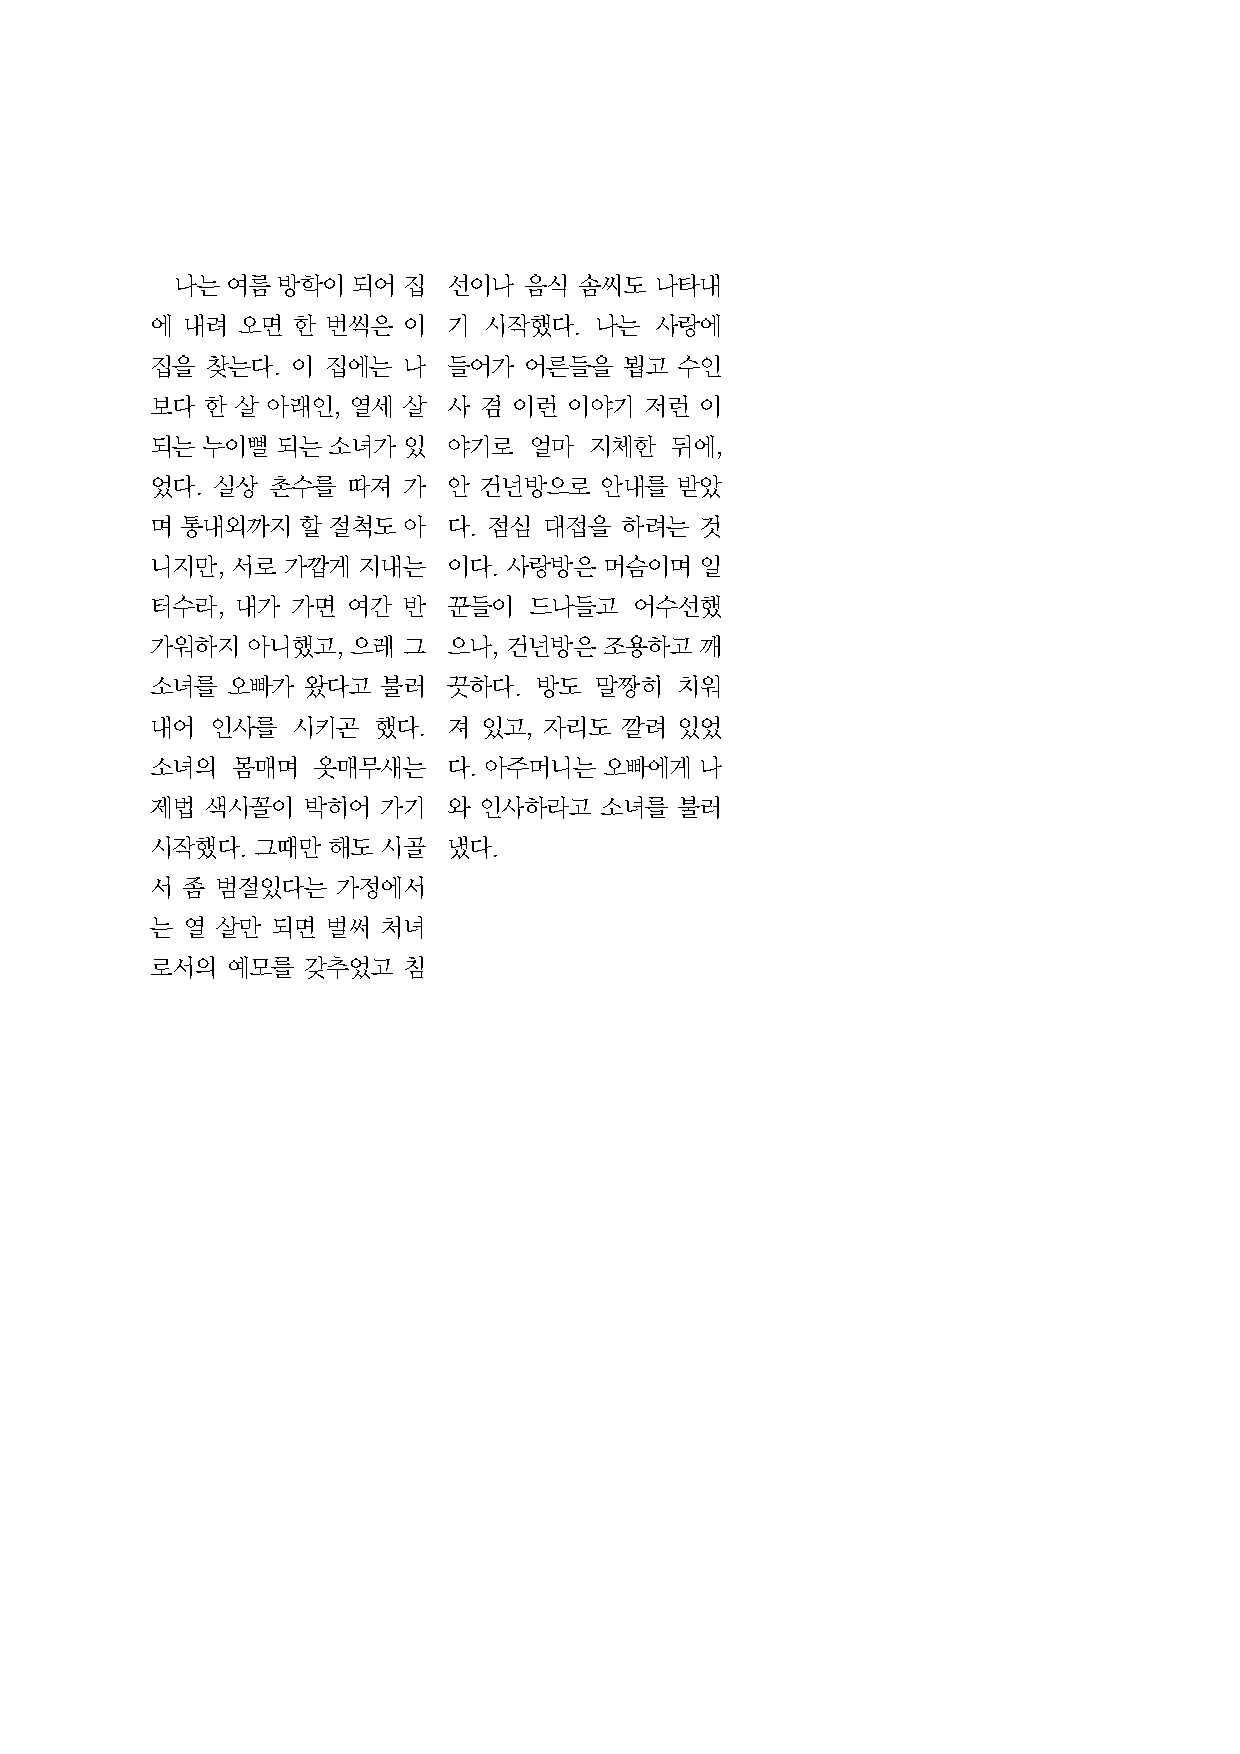
\includegraphics[width=.48\textwidth]{fntnormal}\hfill
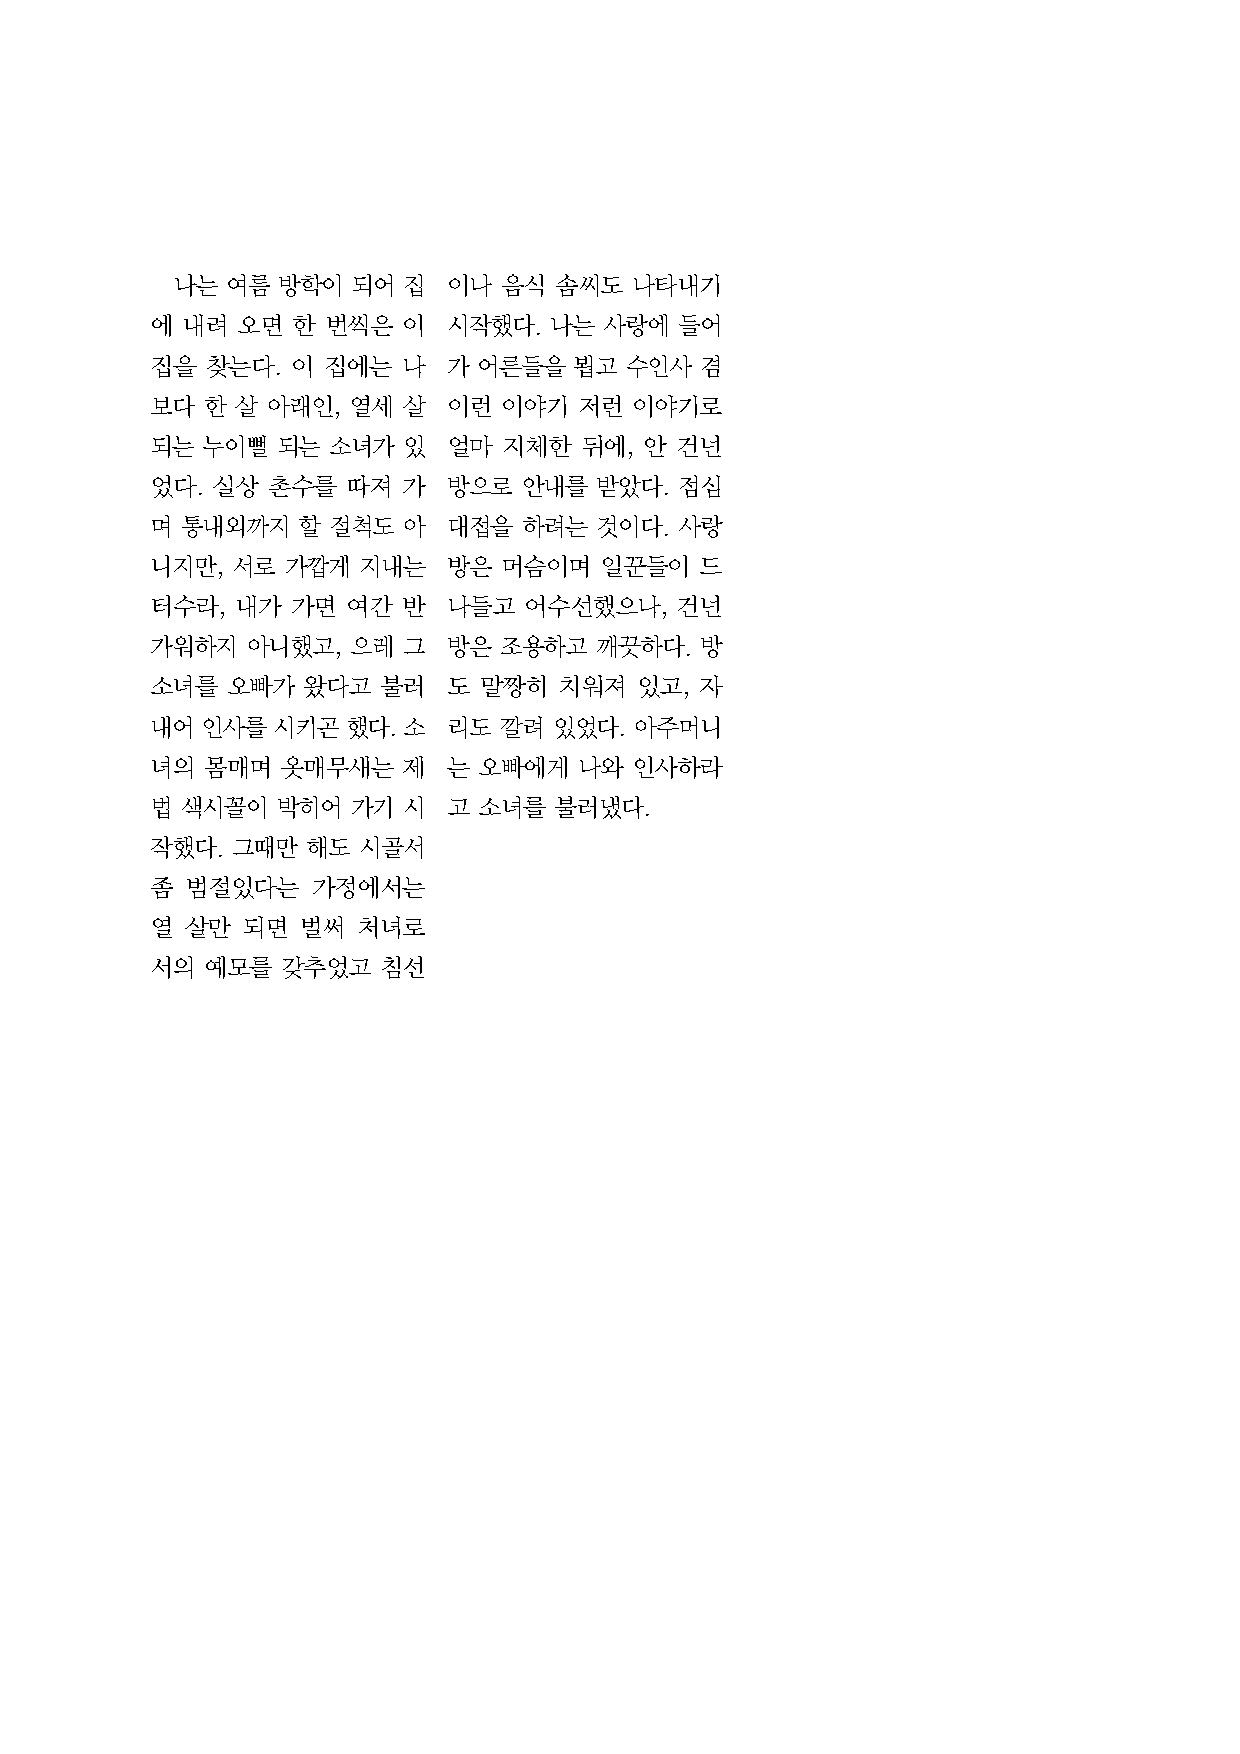
\includegraphics[width=.48\textwidth]{fntexp}\\
\parbox{.48\textwidth}{\centerline{\sffamily\small font expansion 적용 안함}}\hfill
\parbox{.48\textwidth}{\centerline{\sffamily\small font expansion 적용}}
\caption{Font Expansion}\label{fig:fontexpansion}
\end{figure}

샘플 문서의 소스 중에서 font expansion과 관련된 부분은 다음과 같다.
\begin{verbatim}
\usepackage[verbose=true]{microtype}
\DeclareMicrotypeSet{dhucsmicro}{encoding=LUC}
\UseMicrotypeSet[expansion]{dhucsmicro}
\end{verbatim}

\section{행나눔}\index{행나눔}

한글에는 하이픈이 없고 일부 문장부호의 금칙처리를 제외하고는
원칙적으로 모든 문자 앞이나 뒤에서 행을 나눌 수 있다.

\subsection{영문자와 숫자 뒤의 한글 개행}

그림~\ref{fig:allowbreakproblem}에서 표시한 곳은 원본에 영문과 조사가 붙어 있는 부분이다.
빨간색 동그라미 부분에서 영문 단어가 \wi{overfull}이 발생했음에도 불구하고 
뒤에 붙는 한글 조사와 분리되지 않아서 ``\verb|에|''까지 오른쪽으로 
삐져나가 있다. 종래 한글 라텍에서는 이러한 문제가 자주 발생하여
문서작성자를 괴롭히곤 했다.

\begin{figure}
\centering
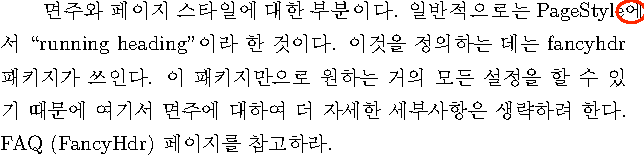
\includegraphics{linebreaktest}
\caption{행나눔 문제}\label{fig:allowbreakproblem}
\end{figure}

\kotex 은 개선된 \wi{행나눔} 기능이 작동한다. 그림~\ref{fig:allowbreakdone}\는
\kotex 을 사용했을 때 이 부분이 어떻게 처리되는가 보여준다.

\begin{figure}
\centering
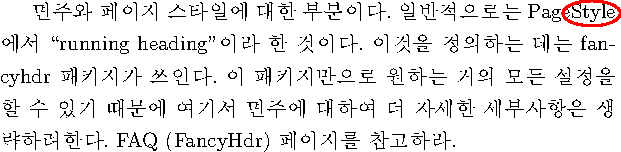
\includegraphics{allowbreak-dhucs}
\caption{dhucs의 행자름 처리}\label{fig:allowbreakdone}
\end{figure}

\subsection{여는 괄호 앞의 행자름}

\wi{여는 괄호}와 관련해서 다음을 지적해둔다. 현재 여는 괄호는 영문자 뒤에 직접
이어서 나오지 않는 한 새로운 줄을 시작할 수 있다. \wi[인명]{신정식} 님께서 알려주신 바에
의하면\footnote{\url{http://www.ktug.or.kr/jsboard/read.php?table=ktugbd&no=4825}}
모든 종류의 여는 괄호는 새로운 줄을 시작하는 것이 유니코드 표준이라고 한다.
그러나 영문으로 글을 쓸 때는 여는 괄호 앞에 하나의 공백을 두게 되어
자연히 새로운 줄을 시작할 수 있을 것이므로 영문자 사이의 여는 괄호를
개행가능하게 하여야 할 필요를 발견하지 못하였다. 그러나 한글과 영문이
만나는 곳에서는 행나눔이 가능하여야 한다. 그림~\ref{fig:openingparen}\을
보라.

\begin{figure}
\centering
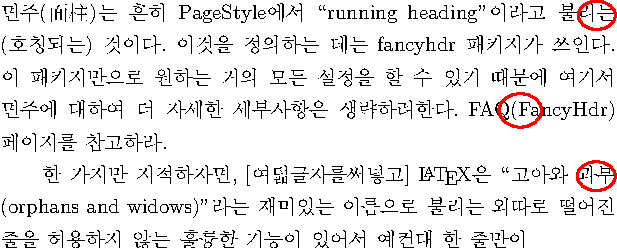
\includegraphics{testdhucsallowbreak}
\caption{여는 괄호의 행자름}\label{fig:openingparen}
\end{figure}

만약 이 그림에서 ``FAQ(FancyHdr)''의 괄호 사이에서 행을 잘라야 한다면
여는 괄호 앞에 공백을 두어
\verb*|FAQ (FancyHdr)|와 같이 써야 할 것이다.

이밖에, \kotex 은 한글 단어 뒤에 괄호 안에 영문을
병기하는 경우 이 영문이 행끝에 걸리더라도 영문 하이픈처리가 작동하도록
하고 있다.

\subsection{이른바 ``고아'' 문제}

``고아''란 한 문단의 마지막 행이 한 글자와 종지부호로만 끝나는 경우를
일컫는다. 한 행 전체 길이에 비교해보았을 때 한 글자 한 행은 그 비중이
너무 작아서 때때로 글읽기의 효율을 방해하고 불필요한 공백이 생겨나게 하여
판면의 색조를 옅게 만드는 것으로 생각되어, 일찍부터 한글 조판의
금기 사항 중 하나였다.\footnote{%
  영어권에서 `고아와 과부'라고 할 때는 이와 조금 다른 의미로 쓰이는
  경우도 있다. 예컨대 Peter Wilson의 \cite{memman}, p.~29에는
  ``\emph{고아}란 한 페이지의 마지막에 한 줄 또는 두 줄이 남는 것을 말한다. 
  Bringhurst의 암기를 위한 트릭에 따르면,
  `고아는 미래만이 있고 과거가 없는 것'이다.''라고 쓰고 있다.
  즉, 과부와 고아가 모두 행나눔에 관한 문제가 아니라
  페이지 나눔에 관한 문제로 취급되고 있는 것이다. 그러나
  이 글에서는 우리나라의 관행적 명칭인 `문단 끝 한 글자 한 행'을 (편의상)
  고아라고 부르기로 한다. 
}

\kotex 에서는 고아 회피가 부분적으로 자동화되었다. 원칙적으로
문단 마지막에 아무런 추가 코드 없이 \verb|\par| 또는 문단 종지 문자가
있을 때는 고아 앞에서 \verb|\nobreak|가 작동하는 것과 같은 효과를
가진다. 그러나 문단 끝에 추가적인 코드나 문자가 더 있을 때 때때로
이 자동 고아 회피가 동작하지 않는 경우도 있으므로, 이럴 때는 
\texttt{\textbackslash nobreak}를
사용자가 직접 지정하여야 한다. 특히 문단의 마지막 글자가 ``다.''일 경우에
한하여 사용자가 고아 회피를 강제하도록 ``\verb|\다|'' 매크로가
새로 도입되었다.\footnote{%
  \url{http://kts.ktug.kr/node/204}.
}
각주 안과 같이 문단 종지 문자 없이 문단이 종료됨으로써
자동 \wi{고아 회피}가 동작하지 않는 경우에
이 매크로를 적절하게 활용할 수 있다.

비록 모든 경우에 완전한 고아 회피가 적용되는 것은 아니지만, 
이만큼이라도 자동화됨으로써 한글 문서 조판의 관행적 규약에 더 가까이
접근했다 하겠다.

\section{한글 PDF 만들기}\label{sec:pdf}

\pageref{sec:makepdf} 페이지 \ref{sec:makepdf}절에서
pdf 제작에 관한 사항을 개괄하였다. 여기서는 이 문제에 대하여
\kotex/utf의 관점에서 조금 더 다루려고 한다. 

한글 pdf 문서를 만드는 데 있어서 지금까지 요청되어 왔던 것은 대략
다음과 같\다.
\begin{itemize}
\item 한글 텍스트의 검색과 추출
\item pdf bookmark에 한글 구현
\item beamer 등 발표 문서 작성 패키지 지원
\end{itemize}

\subsection{하이퍼링크}\label{sec:hyperref}
하이퍼링크를 구현하기 위해서는 \pkg{hyperref}\를 이용한다.
이 패키지 사용에서 주의할 점은 한글 레이블이나 참조자를
사용하면 아니된다는 것이다.

hyperref 설정은 다음 세 가지 방법으로 이루어진다.
\begin{enumerate}
\item\label{itm:one} \verb|\usepackage[...]{hyperref}|의 옵션
\item\label{itm:two} \verb|\hypersetup| 문장
\item\label{itm:three} \file{hyperref.cfg}에 미리 설정된 옵션
\end{enumerate}
예컨대 한글 문서를 주로 작성하는 경우 hyperref의 \texttt{[unicode]}
옵션이 필요하다. 그리고 클래스 자신이 hyperref을 스스로 로드하는
경우에는 (\ref{itm:one})이나 (\ref{itm:two})\과 같은 방법으로
이 옵션을 활성화할 수 없게 되어 있는 경우가 있다. 이럴 때는 (\ref{itm:three})
방법을 사용한다. 즉 \file{hyperref.cfg}에 (\ref{itm:two})의 문장을
미리 적어넣어두는 것이다.

\subsection{폰트 문제}

pdf를 제작하는 방법에 따라
사용할 수 있는 폰트와 그래픽 포맷에 제약이 있다. 
이것을 요약한 것이 표~\ref{tab:pdfdriver}이다. 물론 pk 비트맵 폰트로
변환하면 (pk 생성 유틸리티가 있기만 하다면) 모든 형식의 폰트를 사용할 수 있다 할 것이나,
여기에서는 고품위 pdf를 위한 윤곽선 글꼴의 사용만을 문제삼기로 한다.

\begin{table}
\centering
\caption{dvi to pdf drivers}\label{tab:pdfdriver}
\begin{tabular}{c|cccc|c}
\hline
driver & type1 & truetype & ttf slanted & opentype & graphic \\ \hline
dvips & O & X & X & X & eps \\ 
pdf\TeX & O & O & X & X & pdf/png/mps/jpg \\
DVIPDFM$x$ & O & O & O & O & (eps)/pdf/jpg/png/mps \\ \hline
\end{tabular}
\end{table}

\thispkg의 기본 글꼴은 은 글꼴 type 1이므로, 폰트 이용상의
제약이 전혀 없다. 트루타입을 사용하려 하는 경우라면 표 \ref{tab:pdfdriver}\가
참고가 될 것이다.

\subsection{pdf 한글 텍스트의 검색과 추출}
pdf 파일을 제작하려 할 때 텍스트의 검색과 추출은 매우 중요한
문제 가운데 하나이다. 특히 개방적인 공개 문서의 작성이나 배포,
검색 엔진에서의 검색 가능성 등을 위해 한글 텍스트가 검색 가능하여야
한다. \KTUGFAQ[PDFExtraction]{검색과 추출}
페이지를 참고하라.

DVIPDFM$x$를 이용하면 이 문제를 쉽게 해결할
수 있다. \kotex 으로 작성한 pdf 문서는 DVIPDFM$x$로 pdf 변환한
경우 특별히 텍스트 검색과 추출을 제한하지 않으면 기본적으로 
검색\cntrdot 추출이 이루어진다.

그런데, pdf\LaTeX 는 사실상 표준일 뿐 아니라 pdf\LaTeX 이
아니면 안 되는 경우도 더러 존재한다. 
pdf\TeX\ 최근 버전은 포스트스크립트 type 1 폰트의 경우
유니코드 한글 텍스트의 검색과 추출이 가능하다. 이미 말한 대로,
다음과 같은 코드가 있으면 된다.
\begin{verbatim}
\ifpdf
 \input glyphtounicode\pdfgentounicode=1
\fi
\end{verbatim}
그러나 트루타입 폰트에 대해서는 약간의 문제점을 가진다.

부가 패키지 \pkg{dhucs-cmap}\은 
이 문제를 해결하기 위한 것이다. 따라서 pdf\LaTeX 을 이용하고
트루타입 폰트인 경우 preamble에 다음과 같이 적어준다(여기서는
은 글꼴 트루타입을 예로 들겠다).
\begin{verbatim}
\usepackage{dhucs-cmap}
\pdfmapfile{=unttf-pdftex-kotex.map}
\end{verbatim}
위의 문장은 반드시 \thispkg\를 로드한 \emph{이후에} 선언해야 하고
그렇지 않으면 효력이 없다. 
두번째 행은 은 글꼴을 pdf\LaTeX 에게 트루타입 형식으로 이용하도록 알려주는
것이다. 이 행을 생략하면 pk 비트맵 폰트를 만들어 이용하게 되므로 바라는
결과를 얻지 못할 수 있다. 만약 본문에서 사용하고자 하는 글꼴이 \kotex{}
추가 폰트로 배포되는 
은 글꼴 트루타입이 아니라 별도로 제작한 것이라면 자신의 폰트 설정을 적절한 방식으로 선언해 주어야 한다.
\verb|\pdfmapfile|의 인자로 주어지는 map 파일의 이름 앞에 붙은 \verb|=|는
이미 해당 엔트리가 다른 map에서 스캔되어 있을 때, 지정된 map 파일의
엔트리로 교체하라는 의미이다. \verb|+|를 지정하면 기존의 map 파일에
만약 해당 항목이 스캔되어 있다면 기존의 것이 사용되고 경고 메시지를 낸다.
이에 관한 사항은 pdf\TeX\ 문서를 참조하라.

\subsection{한글 책갈피}\index{pdf bookmark}
pdf 문서 제작에 있어서 한글 책갈피(bookmark)가 필요하면,
다음과 같이 한다.
\begin{verbatim}
\usepackage[unicode,<driver>,...]{hyperref}
\end{verbatim}
\pkg{hyperref}의 개선이 이루어짐에 따라, 한글 책갈피를 만들기 위해
별도의 복잡한 조치를 취할 필요가 없게 되었다. 다만, \verb|<driver>|를
명시해주어야 한다는 데 주의하면 된다. \verb|pdftex|, \verb|dvipdfm|,
\verb|dvips| 등을 지정한다.\footnote{%
  혹 예전 hangul-ucs에서 제작한 문서에서 \pkg{dhucs-ucshyper}\를
  쓰는 경우가 있다면 이것을 \pkg{hyperref}\을 이용하는 방식으로
  소스를 수정하여야 한다. 이 패키지는 더이상 존재하지 않는다.}

\section{찾아보기와 참고문헌}

\wi{색인}(찾아보기, index)을 만들기 위해 제공하는 유틸리티
\file{komkindex.pl}의 사용법에 대해서는 \pageref{sec:komkindex}
페이지 \ref{sec:komkindex}절을 보라. 이 유틸리티와 더불어
한글 색인 스타일인 \verb|kotex.ist|를 제공한다.\footnote{%
  \kotex/euc에는 \texttt{hind.ist}가 제공된다.
  이 둘은 호환가능하지 않으므로 \kotex/utf 문서라면
  반드시 \texttt{kotex.ist}를 색인 스타일로 지정해야 한다.}

\wi{문헌목록} 인용은 가능하다. Bib\TeX 을 이용하여
문헌목록 데이터베이스에서 문헌목록을 추출할 수도 있다.\footnote{%
  다만, 한글화된 문헌목록 스타일이 충분하지 않아서,
  최종적으로 약간의 수작업이 필요한 경우도 없지는 않다고 생각한다.
  특히 저자-연도 방식의 인용에서 그러하다. 이 분야는
  더 많은 연구와 개발이 필요한 지점이다.}

%여기서는 plain 형식의 인용을 테스트해보자.
%즉, \cite{dhhangul} 또는 \cite{yeonam}\과 같은 형식의 문헌 인용이
%가능한 것을 볼 수 있다.

%\begin{quote}
%\cite{dhhangul}\을 보라. \cite{karnes}\를 읽어보라.
%\end{quote}

\wi{참고문헌} 인용은 너무나 많은 유형이 있어서 어떤
문제가 발생할 수 있는지를 완전히 시험해보지 못하였다.
그러나 \pkg{natbib}, \pkg{cite}\와 \pkg{apacite}\을 위한
코드를 내장하고 있어, 참고문헌 인용에서 발생하는 문제에 대한
지원을 위해 노력하고 있다.\footnote{%
  한 예로, \pkg{apacite} 충돌 문제의 보고와 그 해결에 관한
  \href{http://www.ktug.or.kr/jsboard/read.php?table=operate&no=21183}{KTUG 게시판 4984}
  이하의 글타래를 참조하라. 이런 과정을 거쳐서 현재
  \pkg{apacite} 등의 패키지에 대한 지원이 이루어지게 되었다.}

\section{옛한글 구현}\index{옛한글}

옛한글 문서의 조판은 한글 \TeX 의 꿈이었고, KTUG에서 2002년 이후
dhhangul과 같은 Lambda 패키지를 통하여 성공적인 실험을 행한 바가
있다.

현재 이른바 ``한양PUA'' 코드, 즉 유니코드 사용자 영역의 코드를 이용하여
옛한글 문자를 식자하는 것은, 이 영역에 완성형 옛한글 문자가 들어 있는
폰트를 지정하고 해당 코드를 입력하는 것으로 dhucs가 이미
잘 처리한다.\footnote{%
  이 매뉴얼에서는 언급하고 있지 않으나, 현재의 hangul-ucs는
  이미 BMP 영역을 넘어서는 UCS4 문자를 식자할 준비를 갖추고
  있다. 적절한 폰트와 입력코드만 있다면 유니코드 전 영역 문자의
  식자가 가능하다.}
그러나 이것은 엄밀한 의미에서 옛한글 문헌의 조판이라고는 말할 수 
없다.

\pkg{dhucs-midkor}\는 옛한글, 즉 1933년 이전 표기법 문헌을
식자할 수 있게 한다. 그러나 배포판의 매크로만으로 충분하지 않으며,
다음과 같은 준비가 더 필요하다.
\begin{enumerate}
\item 옛한글 폰트(\file{obatang.ttf} 또는 \file{ogulim.ttf})
\item 옛한글 코드 변환 유틸리티
\item 옛한글 코드를 다룰 수 있는 편집기와 입력기
\end{enumerate}

옛한글 문헌의 조판을 위해서 갖추어야 할
조건이 제법 까다롭고\footnote{%
  특히 옛한글을 처리할 수 있는 공개 폰트가 전혀 없다는 점은
  매우 치명적이다.}
이를 처리하는 과정이 편리하다고 할 수 없다\footnote{%
  코드 변환과 같은 약간의 전처리가 필요하다.}%
고는 하나, 옛한글 문헌의 식자를 구현하고 있다는 자체가 매우 중요한 사실이다.
옛한글 조판에 관한 전반적인 사항, 이론적 배경과 구체적인 지침은 \cite{LeeKH}\을
참고하라.\footnote{%
  KC2007의 예제 문서에 옛한글 처리에 관련된 샘플이 포함되어 있다.}

\section{다른 패키지 및 클래스와의 호환성}

\subsection{\texorpdfstring{\AmS-\LaTeX}{AmS-LaTeX} 클래스}
\pkg{amsmath}\를 \LaTeX\ 표준 클래스와 함께 쓰는 경우에는
아무 문제가 없지만 
\cls{amsart}, \cls{amsbook}\과 같은 \AmS-\LaTeX{} 클래스로
문서를 만들 때 한글을 사용하고자 한다면 부딪치는 문제가 몇 가지
있었다. \cls{amsart}의 경우는 다음과 같이 한다.
\begin{Verbatim}[fontsize=\small]
\renewcommand\uppercasenonmath[1]{}
\usepackage{dhucs}
\end{Verbatim}

\cls{amsbook}\은 \verb|\uppercase|가 아스키 코드에 대해서만
동작하기 때문에 발생하는 문제가 있는데, 이를 위하여 다음과 같은
코드를 필요로 한다.
\begin{Verbatim}[fontsize=\small]
\renewcommand\uppercasenonmath[1]{}
\makeatletter
\def\@makechapterhead#1{\global\topskip 7.5pc\relax
  \begingroup
  \fontsize{\@xivpt}{18}\bfseries\centering
    \ifnum\c@secnumdepth>\m@ne
      \leavevmode \hskip-\leftskip
      \rlap{\vbox to\z@{\vss
          \centerline{\normalsize\mdseries
              \MakeUppercase{\chaptername}\enspace\thechapter}
          \vskip 3pc}}\hskip\leftskip\fi
     #1\par \endgroup
  \skip@34\p@ \advance\skip@-\normalbaselineskip
  \vskip\skip@ }
\makeatother
\end{Verbatim}
이 문제는 \cls{amsbook}\이 영어 이외의 언어를 표시하는 문자에
대해 배려하지 않아서 발생하는 것이므로, 위와 같이 수정하여 쓰는
것이 정당하다 할 것이다.

\subsection{beamer 지원}
\pkg{beamer}를 이용하여 PDF 발표 문서를 만들 때는, 다음과 같이
한다. 또는 간단히 \verb|[unicode]| 옵션만 지정해도 될 것이다.
\kotex 에서는 \verb|[nojosa]| 옵션을 주어야 할
필요가 사라졌고, 따라서 \pkg{beamer} 등에서도 자동조사가 잘 작동한다.
\begin{Verbatim}[fontsize=\small]
\documentclass[hyperref={pdftex,unicode}]{beamer}
\usepackage{dhucs}
\end{Verbatim}
\pkg{beamer} 문서는 원칙적으로 pdf\LaTeX 으로 컴파일하여야 한다.

\subsection{prosper/powerdot 지원}
종래 \pkg{prosper}\는 pdf 북마크를 \pkg{hyperref}\을 통해서 만들지
않았기 때문에 한글 북마크의 구현이 쉽지 않았다.
\pkg{hyperref}\를 이용하는 최근의 \pkg{prosper} 또는 \pkg{newprosper}\라면
다음과 같이 하여 북마크를 넣을 수 있다.
\begin{enumerate}
\item \file{prosper.cls}가 \pkg{hyperref}\를 로드할 때 \verb|[unicode]| 
옵션이 활성화되도록 설정한다. 이 옵션은 \verb|hyperref|에서 가장
먼저 주어지는 것이어야 하는데, 시스템의 \file{hyperref.cfg}에
\verb|\hypersetup{unicode=true}|를 선언해두는 것이 가장
손쉬운 방법이다.
\item 글꼴은 type 1 글꼴을 이용한다. \kotex 은 이미 type 1 글꼴이
기본 글꼴로 되어 있으므로 이 문제는 걱정할 필요 없다.
\end{enumerate}

preamble은 다음과 같은 형식이 될 것이다.
\begin{Verbatim}[fontsize=\small]
\documentclass[ps2pdf.....]{prosper}
\usepackage{dhucs}
\SetHangulFonts{utbt}{utgt}{uttz}
\usepackage[dvips,unicode]{hyperref}
\end{Verbatim}

prosper에서 발전한 \pkg{powerdot}\는 한글 사용에 문제가 없다.
다만 이 두 패키지는 모두 dvips, ps2pdf 방식으로 pdf 파일을
제작한다는 점만 염두에 두면 된다.


\section{일본어와 중국어 문단}\index{일본어 문단}

\thispkg\ 2.6 이후 버전은 \pkg{dhucs-trivcj}\을 포함하였다.
이것은 한글 문서에서 약간의 \wi{일본어} 또는 \wi{중국어} 인용문을 처리하게 하려는
목적으로 제작된 것으로서 본격적인 \wi{다국어 문서}를 처리하는 데는 아직
미흡하지만 크지 않은 규모의 일본어 중국어 문단은 나쁘지 않은 정도의
결과를 얻을 수 있을 것으로 생각하고 있다.
일본어 한자의 독음을 작은 가나 문자로 붙이는 것(루비)은 \pkg{CJK}의
일부인 \pkg{ruby}\를 불러서 할 수 있다. 
일본어 또는 중국어 문단을 식자하려면 \pkg{dhucs-trivcj}를
로드하여야 한다.

%\begin{japanesechinese}

\begin{quote}
\begin{japanese}
\LaTeX~というのは、市販ソフト顏負けのきれいな文書が
作れる「文書整形ソフト」で、「ラテック」
もしくは「ラテフ」など変った読み方をします。
ちょっとカタい言葉を使うと「組版~(くみはん)~ソフト」とも言います。
組版とは、活字を組んでページに印刷するための版を作る作業のことで英語で
タイプセッティング~(type setting)~と言います。
\end{japanese}
\end{quote}

일본어와 중국어 글꼴은 \TeX{}Live에 기본으로 포함되어 있는
wadalab-unicode 글꼴과 arphic 글꼴(type 1)을 이용한다. 
\TeX{}Live를 full로 설치하면 당연히 시스템에 설치되어 있을 것이므로
별도의 글꼴 설치 절차 없이 바로 이용할 수 있다.\footnote{%
  KC2006과 같은 시스템에서는 이 글꼴을 설치할 수 있는
  설치 패키지를 별도로 제공할 것이다.}
다만 이 글꼴에는
굵은 글꼴이나 고딕체 글꼴이 별도로 갖추어져 있지 않다.\footnote{%
  Hangul-ucs에서 쓰이던 Adobe Reader의 opentype을
  위한 설정을 사용하기 원한다면, \texttt{dhucs-trivcj-adobe}라는
  꾸러미가 별도로 준비되어 있으므로 그것을 이용하라. 다만 이 때는
  \texttt{\textbackslash usepackage}\texttt{\{dhucs-trivcj-adobe\}}라고
  선언해야 하며, pdf 제작에 DVIPDFM$x$만을 사용할 수밖에 없다는
  점을 기억해두자.}
일본 문자와 로마자가 이어질 때 필요한 `\wi{짧은 간격}'은 tilde(\verb|~|)로 표시할 수 있다.
이것은 \pkg{CJK}의 방식과 동일하다.

\texttt{dhucs-trivcj}가 제공하는 환경은 \texttt{japanese}와
\texttt{chinese}이다. 다만 \texttt{chinese} 환경은 간자체 환경과
번자체 환경을 각각 \texttt{Schinese}와 \texttt{Tchinese}로
구분할 수 있다. 기본값은 \texttt{chinese}가 간자체 환경으로
되어 있지만 만약 번자체 환경을 \texttt{chinese}로 쓰고 싶다면
\begin{verbatim}
\let\chinese\Tchinese
\let\endchinese\endTchinese
\end{verbatim}
라고 선언하면 된다. 다른 문서와의 호환을 위해서 번자체 환경을
그대로 \texttt{Tchinese}라고 쓰는 것도 좋은 방법이다.

다음 표는 \texttt{dhucs-trivcj}에서 사용하는 각 언어별
폰트의 이름이다. 
\begin{center}
\begin{tabular}{l|ll|ll}
\hline
 & \multicolumn{2}{l|}{trivcj} & \multicolumn{2}{l}{trivcj-adobe} \\
\cline{2-5}
 & mj & gt & mj & gt \\
\hline
일본어 & min & -- & jpmj & jpgt \\
중국어간자 & gbsn & -- & cnmj & cngt \\
중국어번자 & bsmi & -- & ctmt & -- \\
\hline
\end{tabular}
\end{center}

간단한 중국어 문장 하나를 식자해보자.\footnote{\url{http://wikka.ctex.org/TeX} 웹사이트에서
인용함.}

\begin{chinese}
\begin{description}
\item[{[}高质量的输出{]}] TeX~遵循传统的排版规则,以排版的质量为最重要的目标。
   如果你把~TeX~的输出结果和用其它的排版软件排版相同的文本所得到的结果加以比较,
   你就会发现其中的区别。
    
\item[{[}超常的稳定性{]}] 自从~TeX~出现以来,只有一些微小的改动。也就是说,
  十几年前的~TeX~文件用现在的~TeX~系统排版得到的结果与十几年前得到的结果是一样的。
  稳定性还体现在~TeX~系统极少会崩溃,可以处理任意大小的文件,即使你的计算机的内存很少,
  TeX~也可自如的工作。
\end{description}
\end{chinese}

%\end{japanesechinese}
\kotex 의 \texttt{dhucs-trivcj}는 pdf\LaTeX, DVIPDFM$x$, dvips
어떤 드라이버로도 잘 처리할 수 있다. 


\chapter{memhangul과 oblivoir}

\section{소개}

\index{클래스!memoir}\index{클래스!oblivoir}%
memoir 클래스는 Peter Wilson 씨가 작성한 것으로 큰 규모의 문서를
조판하는 클래스이다. \LaTeX\ 표준 클래스 중에서는 book이 있는데,
이 book 클래스를 실제 책의 작성에 사용하기 위해 손보아야 할 부분이
상당히 많다. memoir는 book과 비슷한 착상에서 출발했으나, 여기저기서
제안된 book을 수정하는 기능을 하나의 클래스로 합쳐둔 것에 가깝다. 

\pkg{memhangul-ucs}\는 dhucs의 한글 식자 능력을 memoir 클래스에서
이용하기 위해 작성된 것이다. memhangul 자체가 dhucs를 부르며,
그 위에 memoir에 맞는 여러 정의들을 추가하고 있다. memhangul은
원래 독자적인 스타일로 제작되었으나, 2007년 이후 hangul-ucs에
합쳐져 \kotex 으로 계승되었다.
이러한 배경을 가지고 있는 까닭에 oblivoir는 오직 유니코드
한글만을 처리할 수 있으며, EUC-KR 한글 코드로 문서를 작성할
수 없다. 

oblivoir는\footnote{%
  이 이름은 oblivescence(망각)라는 단어와 memoir를
  합쳐서 만든 신조어이다. 원래 memoir 클래스의 memoir는
  논문, 책 등을 의미하는 단어였지만 여기에서는 `기억'이라는
  의미와의 연관성을 고려하여 말장난을 한 것이다.}
memoir 클래스를 이용하면서도 마치 article 클래스의
느낌으로 편리하게 한글 문서를 작성하도록 한 클래스이다. oblivoir는
한글 문서 작성을 목적으로 만들어진 것으로서, 한글화 설정 등을
별도로 할 필요가 없게 되어 있다. 
이 클래스의 의의를 우리는 ``표준적인 한글 문서작성 서식''을
제공하는 데 두었다. 즉, 대부분의 사용자 설정의 기본값을 미리
제공하자는 것이다. 만약 이 기본값에 만족하지 못한다면
memoir 문법으로 손쉽게 사용자화할 수 있게 하고 있다.

dhucs, memoir, memhangul, oblivoir가 상호 의존하는 관계는
그림 \ref{fig:oblivoirtree}에 예시한 바와 같다.

\begin{figure}
\centering
%%%
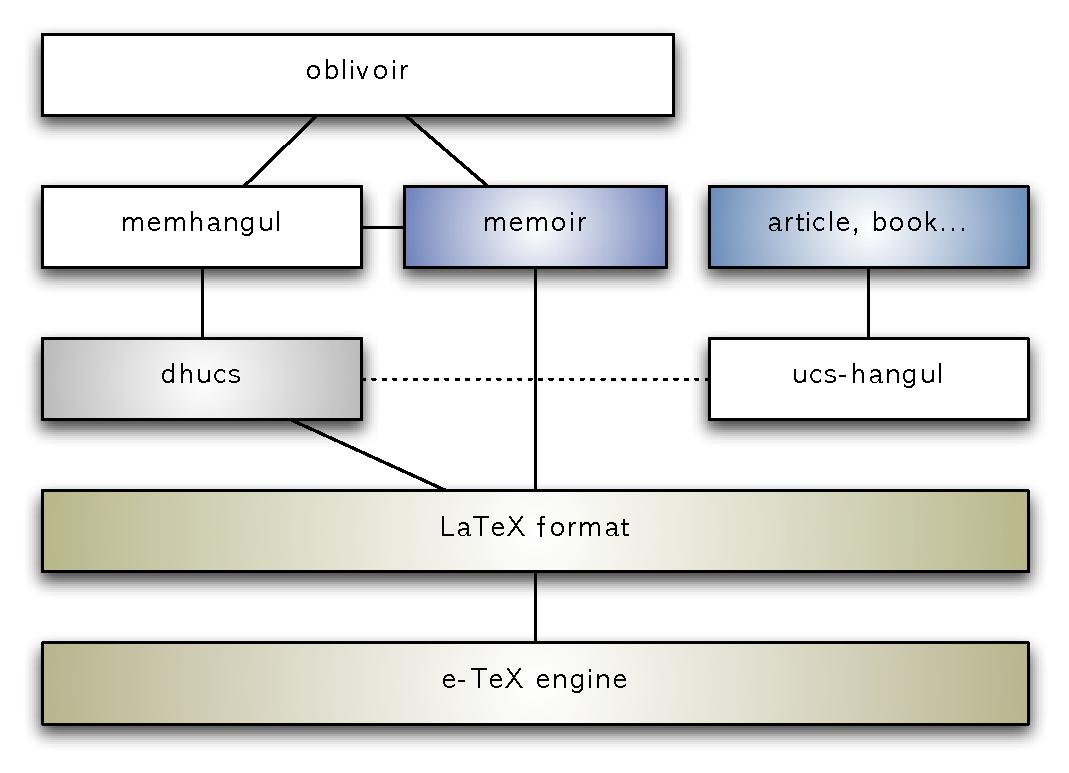
\includegraphics[width=.7\linewidth]{oblivoirtree}
\caption{oblivoir tree}\label{fig:oblivoirtree}
\end{figure}


\section{memhangul}

memoir 클래스 자체가 방대한 기능으로 이루어져 있으며 memhangul 역시
상당한 추가 옵션과 매크로를 가지고 있다. 이 기능을 모두 설명하는 것은
별도의 매뉴얼을 참고하는 것이 좋다. \KTUGFAQ{MemhangulClass} 페이지를
보라. memucs-manual이라는 이름의 한글판 memoir 매뉴얼은 memoir와
memhangul을 이용하려 할 때 필독서이다.
특히 memhangul 패키지에는 한글 타이포그래피를 충족시키기 위한
많은 추가 기능들이 들어 있으며, 이것은 옵션으로 또는 선언으로 조절할
수 있도록 설계되어 있다.

여기서는 간단한 preamble 하나를 예시하는 것으로 만족하려 한다.
\begin{verbatim}
\documentclass{memoir}
\usepackage{memhangul-ucs}
\end{verbatim}

\section{oblivoir}

oblivoir 역시 다양한 옵션과 복잡한 기능을 구현한 설정 패키지들로
이루어져 있다. oblivoir의 사용법 등에 대해서는 \KTUGFAQ{Karnes/Oblivoir/FAQ} 페이지를 참고하라.

\subsection{간단한 문서 만들기}

\begin{verbatim}
\documentclass{oblivoir}
\end{verbatim}

위의 클래스 선언으로 한글 문서를 즉시 작성할 수 있다. pdf\TeX 과 
DVIPDFM$x$ 드라이버는 \verb|pdflatex|으로 컴파일하느냐 \verb|latex|으로
하느냐에 따라 결정되며, dvips 드라이버를 사용하려 한다면 \verb|[dvips]|
옵션을 명시해주면 된다.

oblivoir는 한글 문서 작성시 pdf bookmark를 만드는 것이 default이다.
만약 pdf bookmark를 만들지 않으려 한다면 \verb|[nobookmarks]| 옵션을
명시해준다. 

\verb|[10.5pt]|라는 실험적인 옵션도 있는데, 이것은 본문의 기본 글꼴
크기를 10.5포인트로 맞추어주는 것이다. 10포인트보다는 크고 11포인트보다는
작은 기본 글꼴 크기를 원하는 경우 사용할 수 있다. 또, \verb|\tt, \sf| 같은
\LaTeX\ 2.09 글꼴 명령을 사용하려면 memoir 옵션인 \verb|[oldfontcommands]|를 지시한다.

\subsection{용지, 여백, trim mark}

memoir의 문서 옵션인 종이 크기 옵션 \verb|[a4paper]| 등을 지시하는
것이 가능하다. 이에 더하여, 용지와 여백을 일괄 조정할 수 있는
\pkg{fapapersize}가 제공되는데, 이것은 표준 \LaTeX\ 클래스와는
함께 쓸 수 없고, memoir와 oblivoir에서만 유효하다.

fapapersize 옵션으로 \verb|[dbl4x6]| 또는 \verb|[newmum]| 등을
지정할 수 있으며, 사용자 용지여백 설정 명령인 \verb|\usefapapersize| 명령을
사용할 수 있다.
\begin{verbatim}
\usepackage{fapapersize}
\usefapapersize{*,*,40mm,*,40mm,*}
\end{verbatim}

stocksize를 papersize보다 크게 하면 trim mark를 그릴 수 있다. 이것은
memoir의 trim mark를 이용하는 것이므로 memoir 매뉴얼을 참고하면
쉽게 이해할 수 있다. oblivoir
옵션 \verb|[showtrims]|를 선택하면 된다.

\subsection{글꼴 선택}

본문 글꼴을 선택할 수 있는 명령 \verb|\SelectHfonts|가 제공된다.
사용법은 다음과 같다. 인자는 두 개이며, 첫번째 것은 한글, 두번째
것은 한자 글꼴을 각각 rm/sf/tt에 대하여 쉼표(,)로 구분한다.
\begin{verbatim}
\SelectHfonts{<rm>,<sf>,<tt>}{<rm>,<sf>,<tt>}
\end{verbatim}
\verb|*|를 이용하여 다음과 같이 간략하게 쓸 수 있다.
\begin{verbatim}
\SelectHfonts{kxbt,kxgt,*}{*}
\end{verbatim}

\subsection{기타}

oblivoir는 자체 명령뿐 아니라 memhangul의 명령, memoir의 명령,
\LaTeX 의 명령, \TeX 의 명령을 모두 사용할 수 있다. 위에 소개한 것 말고도
많은 추가적인 기능이 있으므로 매뉴얼을 참고하라.

\endinput
